\documentclass[11pt]{article}
\usepackage{amsmath,amssymb,amsthm}
\usepackage{enumitem}
%\usepackage{nopageno}
\usepackage[left=1in,right=1in,top=1in,bottom=1in]{geometry}
\usepackage{tikz}
\usetikzlibrary{cd,decorations.pathmorphing}
\usepackage{xcolor}
\usepackage{sectsty,wrapfig}
\usepackage{hyperref}


\allsectionsfont{\normalsize}
%\linespread{1.1}

\newtheorem{thm}{Theorem}[section]
\newtheorem{prp}[thm]{Proposition}
\newtheorem{lmm}[thm]{Lemma}
\newtheorem{crl}[thm]{Corollary}
\newtheorem{ques}[thm]{Question}
\newtheorem{fact}[thm]{Fact}

\theoremstyle{definition}
\newtheorem{dfn}[thm]{Definition}
\newtheorem{eg}[thm]{Example}

\theoremstyle{remark}
\newtheorem{rmk}[thm]{Remark}

\def\wt#1{\widetilde{#1}}
\def\ov#1{\overline{#1}}
\def\mr#1{{\mathring{#1}}}


\def\Z{\mathbb{Z}}
\def\C{\mathbb{C}}
\def\P{\mathbb{P}}
\def\R{\mathbb{R}}
\def\Q{\mathbb{Q}}
\def\D{\mathbb{D}}
\def\M{\mathfrak{M}}
\def\cA{\mathcal{A}}
\def\cD{\mathcal{D}}
\def\cM{\mathcal{M}}
\def\cT{\mathcal{T}}
\def\cN{\mathcal{N}}
\def\rI{{\mathring{I}}}
\def\dom{{\tn{dom}}}

\def\cmt#1{\textcolor{purple}{(#1)}}
\def\tn#1{\textnormal{#1}}
\def\pr{{\textnormal{pr}}}
\def\x{\!\times\!}

\begin{document}

\setlength{\parskip}{\baselineskip}
\setlength{\parindent}{0cm}

\section{Basic notion}
\label{basic_sec}

For any $n\in\Z^{>0},\epsilon\in\R^{>0},p\in\R^d$, denote by $\D^n_p(\epsilon)\subset\R^n$ the (closed) $n$-dimensional ball centered at $p$ and of radius $\epsilon$; denote by $\mr\D^n_p(\epsilon)$ its interior. 
If $p=0$ or $\epsilon=1$, we omit it from the notation. 
Denote by $S^{n}$ the standard $n$-dimensional sphere. 

For a topological space $B$ and a continuous function $g: B\to \R^{>0}$, define
$$\cD_B(g)\xrightarrow{\pi^\cD_{B}} B\qquad
(\tn{resp. } \mr\cD_B(g)\xrightarrow{\pi^\cD_B} B)$$
to be the smooth sub-fiber bundle of $\R^d\times B$ such that the fiber over $b\in B$ is $\D^d(g(b))$ (resp. $\mr\D^d(g(b))$). 
Let $\sigma_B^\cD:B\to \cD_B(g)$ (resp. $\mr\cD_B(g)$) be the zero-section. 
Similarly, define
$$\cA_B(g)\xrightarrow{\pi^\cA_B} B\qquad
(\tn{resp. } \mr\cA_B(g)\xrightarrow{\pi^\cA_B} B)$$
to be the smooth sub-fiber bundle of $\R^d\times B$ such that the fiber over $b\in B$ is $\R^d\backslash\mr\D^d(g(b))$ (resp. $\R^d\backslash\D^d(g(b))$). 

Let $d\geq4$ be an integer. Suppose $M$ is a $d$-dimensional $\Z$-homology sphere. 

\begin{dfn}
An {\it ($M,\infty$)-bundle} is a tuple $(\pi:E\to B,\sigma,\tau)$, where
\begin{itemize}
\item $\pi:E\to B$ is a smooth fiber bundle whose fibers are diffeomorphic to $M$;
\item $\sigma:B\to E$ is a smooth section of $\pi$; 
\item $\tau$ is a germ of trivializations of $\pi$ near $\sigma(B)$, namely: 
\begin{itemize}
\item say $(\phi, U,g)$ is a trivialization of $\pi$ near $\sigma(B)$ if 
\begin{itemize}
\item $U\subset E$ is a neighborhood of $\sigma(B)$, $g:B\to\R^{>0}$ is smooth and 
\item $\phi: U\to \mr{\cD}_B(g)$ is a diffeomorphism satisfying 
$$\pi^\cD_{B}\circ\phi=\pi\qquad \phi\circ\sigma=\sigma^\cD_B;$$
\end{itemize}
\item say two such $(\phi_1,U_1,g_1)$, $(\phi_2,U_2,g_2)$ are equivalent if there exists an open subset $U'\subset U_1\cap U_2$ such that $\phi_1|_{U'}=\phi_2|_{U'}$; 
\item $\tau$ is an equivalence class of such trivializations of $\pi$ near $\sigma(B)$. 
\end{itemize}
\end{itemize}
\end{dfn}

For later convenience, given such a $(\phi,U,g)$ in the equivalence class $\tau$, we write $U'=U\backslash(\sigma(B))$, and define 
$$\phi': U'\to\mr\cA_B(1/g)\qquad \phi'=\big((b,x)\to (b,x/|x|^2)\big)\circ\phi|_{U'}.$$
\begin{dfn}
We call such a $(\phi',U',1/g)$ a {\it representative} of $\tau$. 
\end{dfn}

\begin{dfn}
Let $(\pi:E\to B,\sigma,\tau)$ be an $(M,\infty)$-bundle. 
Denote by $T^vE$ the vertical tangent bundle of $E$. 
A {\it framing} $F$ on $\pi$ is a trivialization of $T^vE$ over $E\backslash\sigma(B)$, 
$$F: T^vE|_{E\backslash\sigma(B)}\approx\R^d\times E\big\backslash\sigma(B),$$ 
such that, there exists $(\phi',U',g)$ a representative of $\tau$, such that $\phi'_*(F)$ is the standard framing on $\mr\cA_B(1/g)$. 
\end{dfn}

Given such a framing $F$ and $p\in E\backslash\sigma(B)$, denote by $F|_p:T^v_pE\to\R^d$ the restriction of $F$ to the vertical tangent space at $p$. 

\begin{dfn}
Let $(\pi:E\to B,\sigma,\tau)$ be an $(M,\infty)$-bundle and let $F$ be a framing on $\pi$. 
Define the {\it exponential map}
$$\exp: T^vE|_{E\backslash\sigma(B)}\to E\backslash\sigma(B)$$
as follows. 
Suppose $v\in T^v_pE$. Suppose 
$$F(v)=(v', p)\in \R^d\times E\backslash \sigma(B).$$
Then, $F^{-1}\big(\{v'\}\times E\backslash \sigma(B)\big)$ is a (vertical) vector field on $E\backslash\sigma(B)$, containing $v$. 
Let $\gamma_v:\R^{\ge0}\to E\backslash\sigma(B)$ be the integral curve of this vector field such that $\gamma_v(0)=p$. 
Then, define $\exp(v)=\gamma_v(1)$. 

Given $p\in E$, denote by $\exp_p:T^v_pE\to E$ the restriction of $\exp$ to the vertical tangent space at $p$. 

\end{dfn}



{\bf Fact:} For every $p\in E\backslash\sigma(B)$, there exists $\epsilon>0$, such that, the restriction of 
$$\exp_p\circ (F|_p)^{-1}:\R^d\longrightarrow E$$
to $\D^d(\epsilon)$ is an embedding. 
\cmt{cite some source for this}



For an $(M,\infty)$-bundle $(\pi:E\to B,\sigma,\tau)$, and for a finite set $A$, denote 
$$C_A(\pi)=\{(x_i\in E)_{i\in A}\big|\,\forall i, x_i\notin\sigma(B)\tn{ and }\forall i\neq j,x_i\neq x_j, \pi(x_i)=\pi(x_j) \};$$
it is an open subset of
$\underbrace{E\times_{B}E\times_B\ldots\times_BE}_{A-\tn{times}}$. 
Denote by $\ov{C}_A(\pi)$ its Fulton-MacPherson compactification. 
Abusing notation, we also denote by 
$$\pi:C_A(\pi) (\tn{resp. }\ov{C}_A(\pi)) \longrightarrow B$$
the map of a configuration to the base point the fiber over which the points in the configuration lie on. 

Similarly, denote 
$$C_A(\R^d)=\Big(\underbrace{\R^d\times\ldots\times\R^d}_{A-\tn{times}}-(\tn{the big diagonal})\Big)\Big/\tn{scaling and translations}.$$
Denote by $\ov{C}_A(\R^d)$ its Fulton-MacPherson compactification. 

%\begin{dfn}
%For a configuration $x\in C_A(\pi)$, and $a\in A$, we define $r^{max}_x(a)$ to be
%
%\end{dfn}




\subsection{a choice and more notation}
\label{notation11_sec}

For the rest of this note, suppose we are given two $d$-dimensional $\Z$-homology spheres $M_1,M_2$, an $(M_1,\infty)$-bundle $(\pi_1:E_1\to B_1,\sigma_1,\tau_1)$ with framing $F_1$, and an $(M_2,\infty)$-bundle $(\pi_2:E_2\to B_2,\sigma_2,\tau_2)$ with framing $F_2$. 
Assume $B_1,B_2$ are compact. 

For $i=1,2$, we choose a representative $(\tau'_i,U'_i,g_i)$ of $\tau_i$ and fix this choice for the rest of this document. 
Without loss of generality of all the arguments in this document, we assume $g_i\equiv1$. 
%\begin{itemize}
%\item Choose a representative $(\tau'_i,U'_i)$ of $\tau_i$.  
%\item Choose a fiberwise Riemannian metric on $E_i\backslash\sigma_i(B_i)$, namely, a Riemannian metric on each fiber, varying smoothly as the fiber varies; we require the metric to satisfy the condition that, when restricted to $U'_i$ and pushed-forward by $\tau'_i$, it coincides with the standard metric on $\R^d\backslash\D^d$. 
%\end{itemize}

Some notation: 

\begin{itemize}
\item For $N\ge1$, denote $$E_i(N)=E_i-\Big((\tau'_i)^{-1}(B_i\times\R^d\backslash\D^d(N))\Big)\qquad E_i(N)^{\circ}=E_i-\Big((\tau'_i)^{-1}(B_i\times\R^d\backslash\mr\D^d(N))\Big).$$

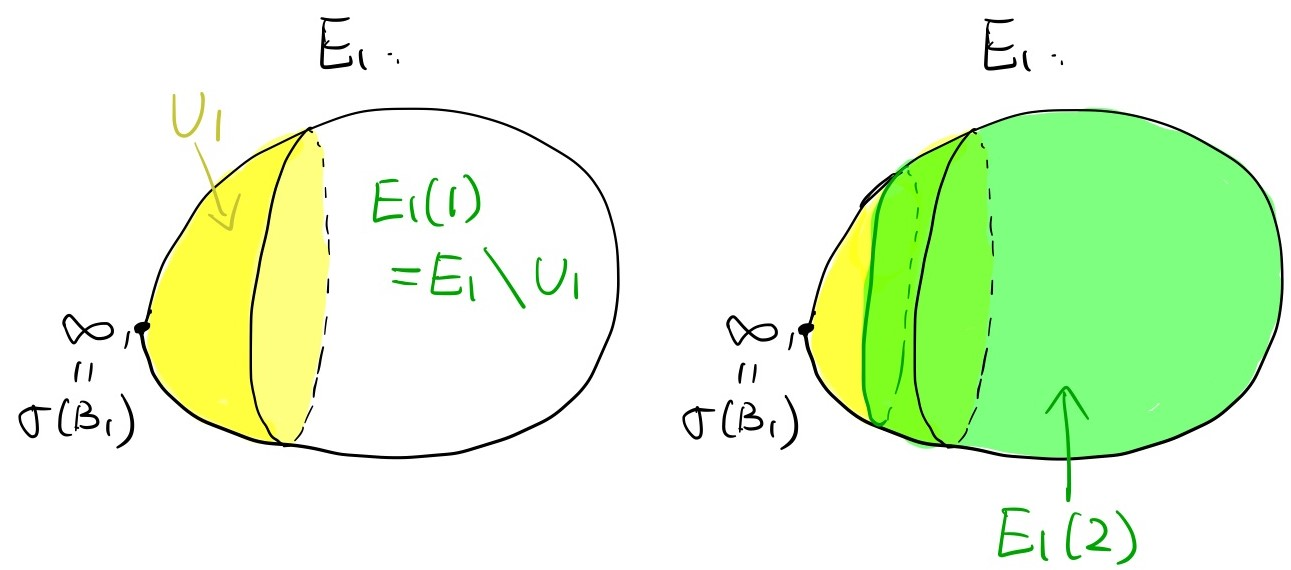
\includegraphics[scale=0.17]{fig1_fig}

\item For $p\in E_i$, define ``$\tn{radius}^{\max}(p)$'' to be the biggest $\epsilon>0$ such that the map 
$\exp_p\circ (F|_p)^{-1}\big|_{\D^d(\epsilon)}$
is an embedding. 
For $0<\epsilon<\tn{radius}^{\max}(p)$, we define \begin{equation}\label{Ddef_eqn}
D_p(\epsilon):=\exp_p\circ (F|_p)^{-1}(\D^d(\epsilon))\subset E_i|_{\pi_i(p)}.
\end{equation}

\item Define $\rho_0=\frac{1}{2}\tn{min}\big(\{\tn{radius}^{\max}(p)\}_{p\in E_1\cup E_2}\sqcup\{1\}\big)$ and $\rho=\frac{1}{4}\rho^2_0$. 
%The motivation is: $2\rho_0$ is the biggest radius of a ``small disk'' near a point in $E_1$ or $E_2$, that can still be viewed as roughly the standard disk; and for safety we often just use $\rho_0$ instead of $2\rho_0$ for this. And $(0,\rho)$ is the the range of the gluing parameter $t$. The purpose of taking $\rho_0^2$ 
\end{itemize}

%On the other hand, given a finite set $A$ with at least 2 elements, and an element $c\in \ov{C}_A(\R^d)$, we define a ``canonical normalization'' of $c$---a choice of an element in $\underbrace{\R^d\times\ldots\times\R^d}_{A-\tn{times}}\big\backslash (\tn{the big diagonal})$, in the equivalence class $c$---as follows: 
%
%
%For a screen, we normalize it (identify it with $\mathbb{R}^d$) by defining 0 to be the center of gravity of the marked points (including nodes), and defining 1 to be the maximal distance between a marked point (including nodes) and 0. Again $B_\epsilon(p)$ denotes the ball of radius $\epsilon$ with center $p$. 


\section{Defining the bracket bundle}
\label{bracketbundle_sec}

In this section, for $0<t<\rho$, we define the bracket bundle, $\pi^t:E^t\to B^t$ ($t$ is the ``gluing parameter''). 

\subsection{Defining the base}\label{Bt_sec}
First, the base $B^t$ is the same space for all $t$, so we call this space $B'$, which we define now. 
It is obtained by gluing together three pieces: \begin{equation}\label{piecesB_eqn}
{E_1(3)^\circ}\times B_2,\quad S^{d-1}\times (-\frac{1}{2},\frac{1}{2})\times B_1\times B_2,\quad B_1\times {E_2(3)^\circ}.
\end{equation}
The gluing is done as follows: 
we glue part of the first piece 
$$({E_1(3)^\circ}-E_1(2))\times B_2 \ \subset\  E_1(3)^\circ\times B_2$$
to part of the second piece 
$$(-\frac{1}{2},-\frac{1}{3})\times B_1\times B_2\ \subset\  (-\frac{1}{2},\frac{1}{2})\times B_1\times B_2$$
using the diffeomorphism
$$(E_1(3)-E_1(2))\times B_2\stackrel{\tau'_1}{\approx} (\mr\D^d(3)-\D^d(2))\times B_1\times B_2\approx S^{d-1}\times(2,3)\times B_1\times B_2\approx S^{d-1}\times(-\frac{1}{2},-\frac{1}{3})\times B_1\times B_2,$$
where the last map is given by 
$$(2,3)\to(-\frac{1}{2},-\frac{1}{3}),\qquad x\to -1/x.$$
Similarly, we glue part of the third piece 
$$B_1\times(E_2(3)^\circ-E_2(2))\ \subset\ B_1\times E_2(3)^\circ$$
to part of the second piece 
$$(\frac{1}{3},\frac{1}{2})\times B_1\times B_2\ \subset\  (-\frac{1}{2},\frac{1}{2})\times B_1\times B_2$$
using the diffeomorphism 
\begin{align*}
B_1\times(E_2(3)^\circ-E_2(2))\stackrel{\tau'_2}{\approx}B_1\times(\mr\D^d(3)-\D^d(2))\times B_2\approx S^{d-1}\times(2,3)\times B_1\times B_2\\
\stackrel{\tn{antipodal map on }S^{d-1}}{\approx}S^{d-1}\times(2,3)\times B_1\times B_2\approx(\frac{1}{3},\frac{1}{2})\times B_1\times B_2,
\end{align*}
where the last map is given by 
$$(2,3)\to(\frac{1}{3},\frac{1}{2}),\qquad x\to 1/x.$$

A picture of $B'$: 
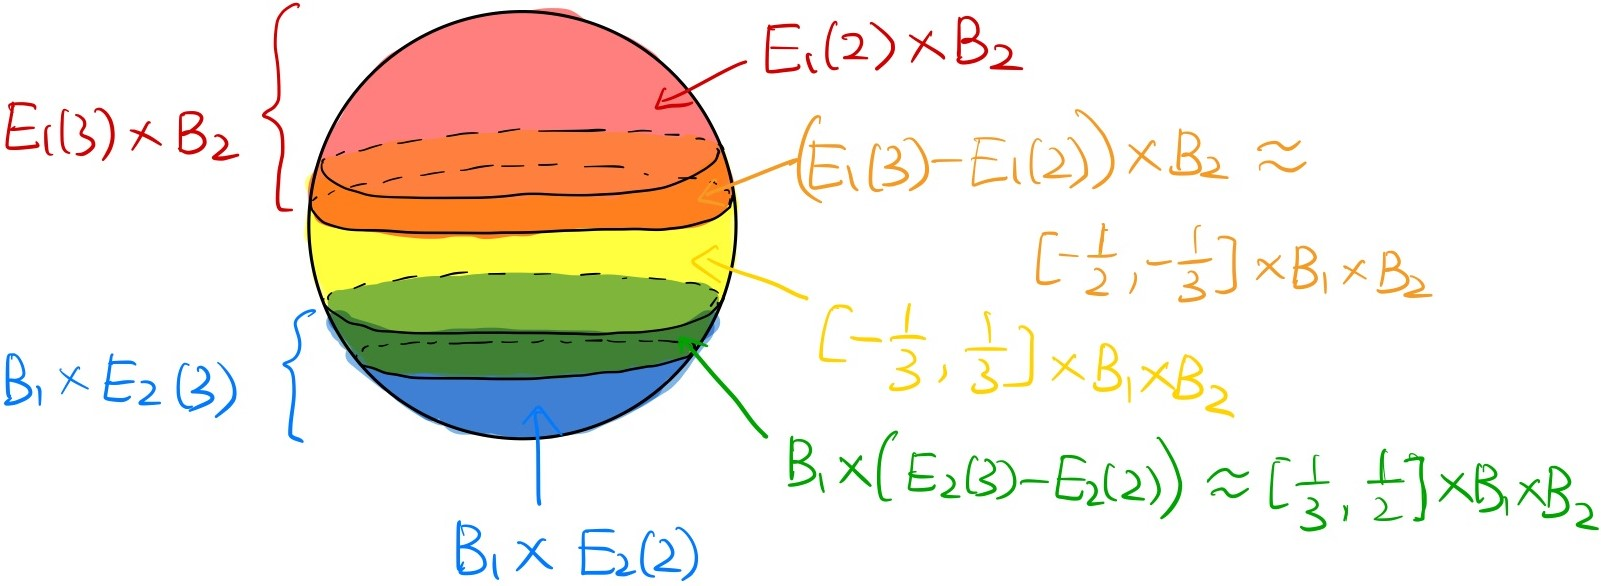
\includegraphics[scale=0.18]{fig2_fig}

\begin{rmk}
The orientation on $B'$ needs a bit of care. 
\end{rmk}


This completes the definition of $B'$. 
We define $B_\rI=B'\times (0,\rho)$, and $\bar\pi:B_{\rI}\to(0,\rho)$ the projection to the second factor. Define $B^t=\bar\pi^{-1}(t)$. 

%Now, given $b\in B^t$, we define the fiber $E^t|_{b}$. 

\subsection{Defining the total space}
\label{EI_subsec}
Now we define a bundle $\pi_\rI:E_\rI\to B_\rI$ that restricts to $\pi^t$ for each $t\in(0,\rho)$. 

\subsubsection{Over the first part of the base}
\label{first_subsubsec}
We first construct $E_\rI|_{E_1(3)^\circ\times B_2\times (0,\rho)}$, as follows: 

Define the tautological bundle $(\pr^1_{B_1})^*E_1\to E_1(3)^\circ\times B_2\times (0,\rho)$ as the pull back bundle
\[\begin{tikzcd}
(\pr^1_{B_1})^*E_1\rar["f_1"]\dar["(\pr^1_{B_1})^*(\pi_1)"] & E_1\dar["\pi_1"] \\
E_1(3)^\circ\times B_2\times (0,\rho)\rar["\pr^1_{B_1}"] & B_1
\end{tikzcd}\]
where $\pr^1_{B_1}$ is by projecting to the first factor and then mapping by $\pi_1$. 
It has a canonical section 
\begin{align*}
s_1: E_1(3)^\circ\times B_2\times (0,\rho)\longrightarrow (\pr^1_{B_1})^*E_1\\
(p,b_2,t)\longrightarrow f^{-1}_1(p);
\end{align*}
here, although $f_1$ itself is not a diffeomorphism, its restriction to each fiber is, and the ``$f_1^{-1}$'' here means the inverse of the restriction of $f_1$ to the fiber over $(p,b_2,t)$. 
For a function 
$$\lambda:E_1(3)^\circ\times B_2\times (0,\rho)\longrightarrow(0,2\rho_0),$$
let 
$$\mathcal{D}(\lambda)\longrightarrow E_1(3)^\circ\times B_2\times (0,\rho)$$ 
be the fiber bundle whose fiber over $(p,b_2,t)$ is $\D^d(\lambda(p,b_2,t))$. 
We have a fiber bundle map 
\begin{align}\label{exp1_eqn}
\mathcal{D}(\lambda)&\longrightarrow (\pr^1_{B_1})^*E_1\\
\big(v\in \D^d(\lambda(p,b_2,t)),(p,b_2,t)\in E_1(3)^\circ\times B_2\times(0,\rho)\big)&\longrightarrow f_1^{-1}\big(\exp_p((F_1|_p)^{-1}(v))\big)\nonumber
\end{align}
which is an embedding. 
Define
$\mathcal{N}(s_1,\lambda)$ to be the image of this map. 
It is a closed neighborhood of the image of $s_1$. 
\cmt{include a better picture?}
For a function $g:(0,\rho)\to(0,2\rho_o)$, define $$\mathcal{D}(g(t))=\mathcal{D}((p,b_2,t)\to g(t)),\qquad\cN(s_1,g(t))=\cN(s_1,((p,b_2,t)\to g(t))).$$
For a constant $c\in(0,2\rho_0)$, define 
$\mathcal{D}(c)=\mathcal{D}(\lambda)$ and $\cN(s_1,c)=\cN(s_1,\lambda)$ where $\lambda\equiv c$ is the constant function. 

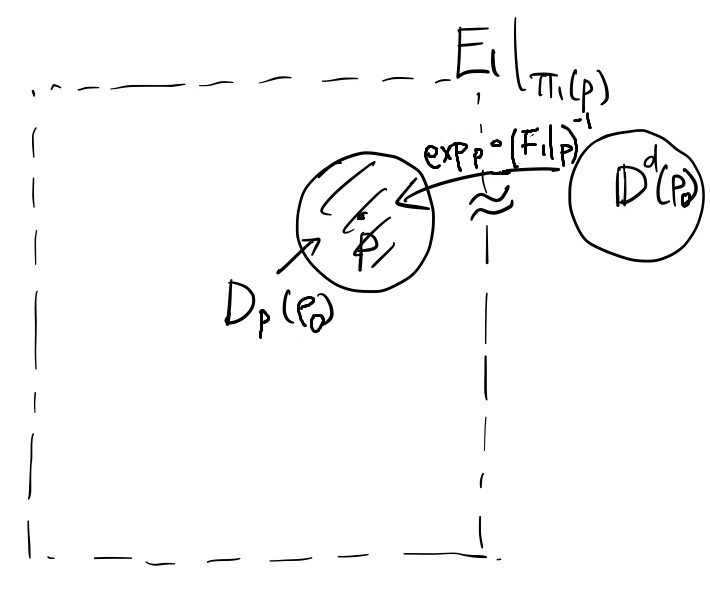
\includegraphics[scale=0.2]{fig3-1_fig}

Define also the following pull-back bundle:
\[\begin{tikzcd}
(\pr^1_{B_2})^*E_2\rar["f'_2"]\dar["(\pr^1_{B_2})^*\pi_2"] & E_2\dar["\pi_2"] \\
E_1(3)^\circ\times B_2\times (0,\rho)\rar["\pr^1_{B_2}"] & B_2
\end{tikzcd}\]
where $\pr^1_{B_2}$ is the projection onto the $B_2$ factor. 
For a function 
$$\lambda:E_1(3)^\circ\times B_2\times (0,\rho)\longrightarrow[1,\infty),$$ 
define $(\pr^1_{B_2})^*E_2(\lambda)$ to be the disk sub-bundle of $(\pr^1_{B_2})^*E_2$ whose fiber over $(p,b_2,t)$ is $E_2(\lambda(p,b_2,t))|_{b_2}$. 
\cmt{include a picture?} 
For a function $g:(0,\rho)\to(0,2\rho_o)$, define $$(\pr^1_{B_2})^*E_2(g(t))=(\pr^1_{B_2})^*E_2((p,b_2,t)\to g(t)).$$

Now, $E_\rI|_{E_1(3)^\circ\times B_2\times (0,\rho)}$ is constructed by removing $\cN(s_1,t)$ from $(\pr^1_{B_1})^*E_1$, and glue back $(\pr^1_{B_2})^*E_2(\rho_0/t)$. 
The gluing is done via the bundle-isomorphism
\begin{align}\label{filling_eqn}
(\pr^1_{B_2})^*E_2(\rho_0/t)-(\pr^1_{B_2})^*E_2(1)\stackrel{\tau'_2}{\approx}(\D^d(\rho_0/t)-\D^d(1))\times E_1(3)^\circ\times B_2\times(0,\rho) \nonumber\\
\stackrel{\tn{scaling by }t}{\approx}\mathcal{D}(\rho_0)-\mathcal{D}(t)\stackrel{(\ref{exp1_eqn})}{\approx}\cN(s_1,\rho_0)-\cN(s_1,t).
\end{align}

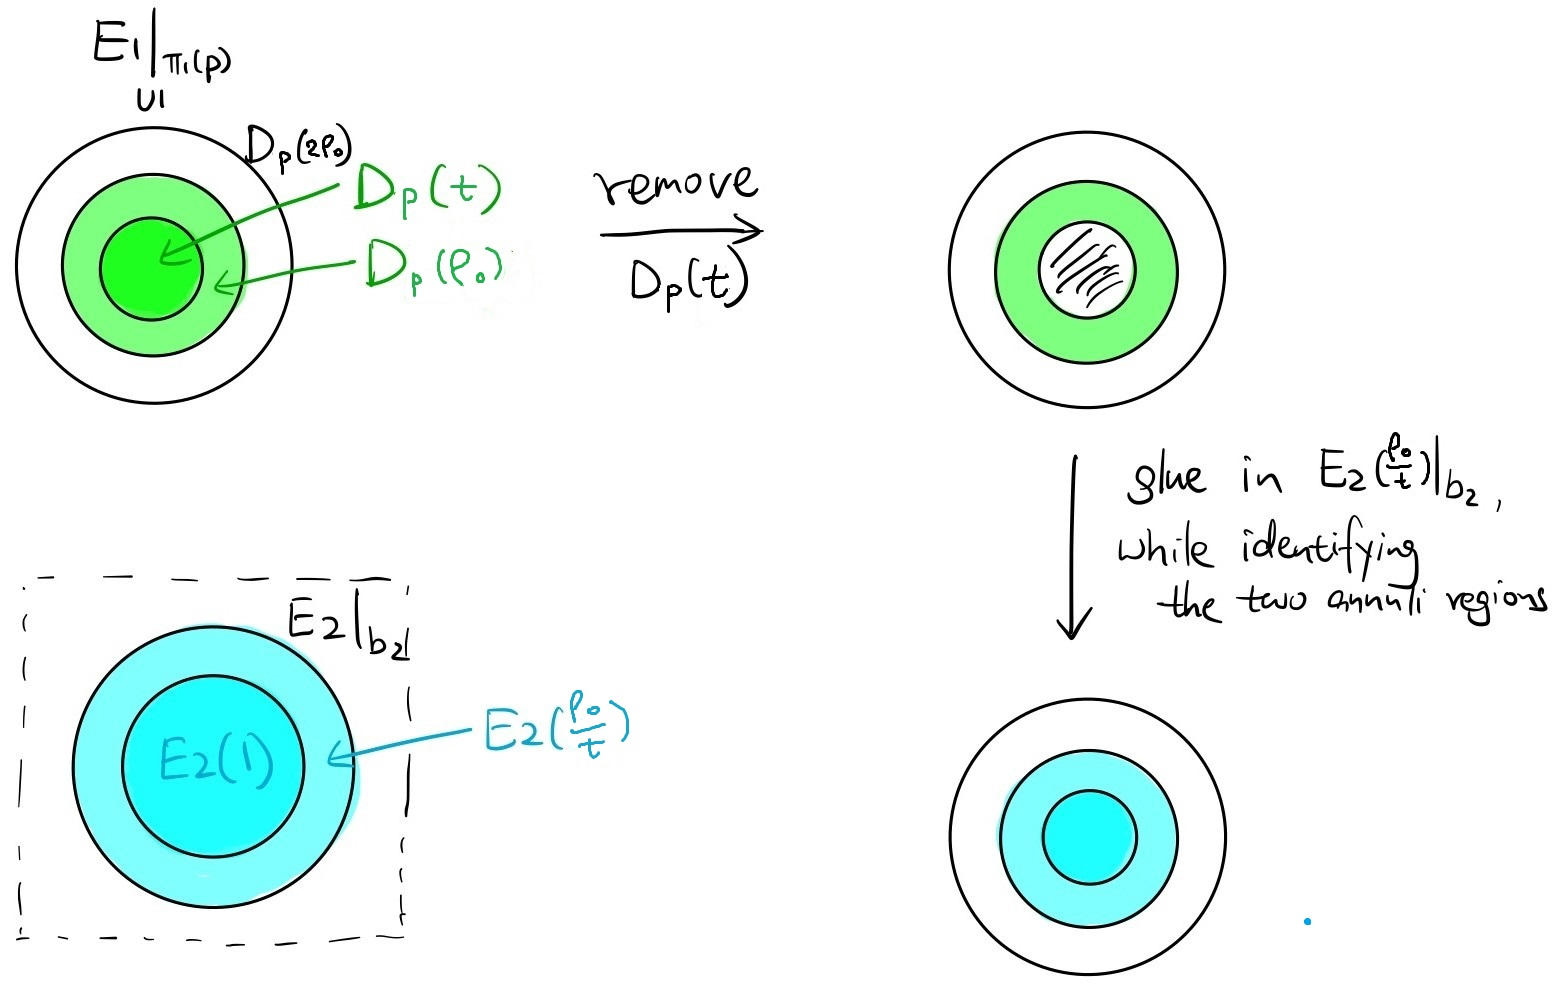
\includegraphics[scale=0.2]{fig3-2_fig}

This completes the construction of $E_\rI|_{E_1(3)^\circ\times B_2\times (0,\rho)}$. Clearly, the projection map
$$E_\rI|_{E_1(3)^\circ\times B_2\times (0,\rho)}\to E_1(3)^\circ\times B_2\times (0,\rho)$$ 
is a submersion. The construction of $E_\rI|_{B_1\times E_2(3)^\circ\times (0,\rho)}$ is similar. 


\subsubsection{Over the second part of the base}
\label{second_subsubsec}
It remains to construct 
$E_\rI|_{S^{d-1}\times(-\frac{1}{2},\frac{1}{2})\times B_1\times B_2\times(0,\rho)}$.
The intuition here is that we gradually increase the size of $E_2(1)$ and decrease the size of $E_1(1)$ in $\R^d$, as the picture below. 

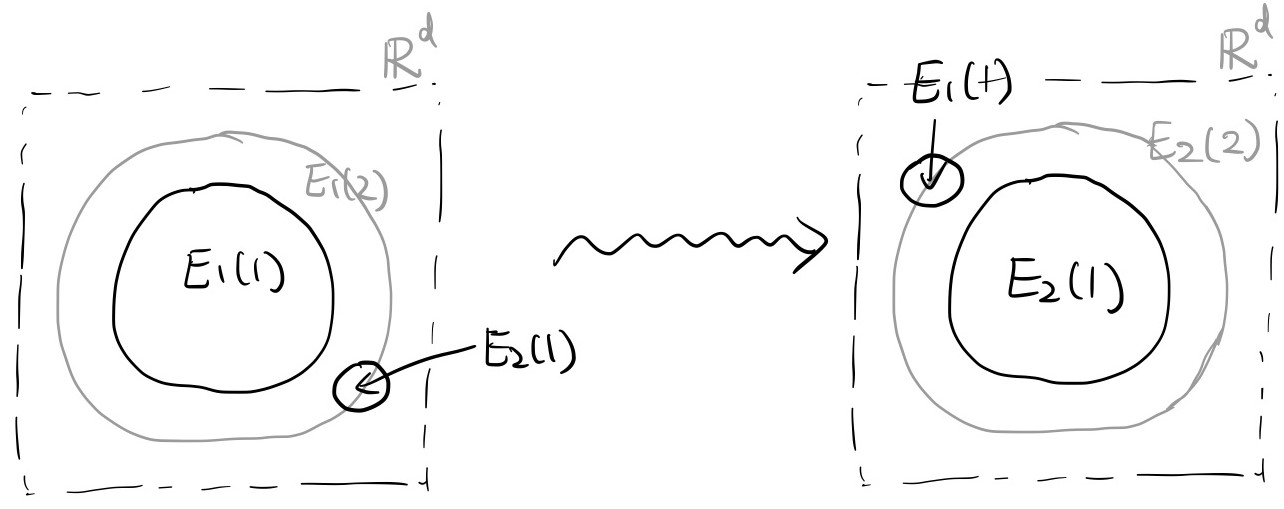
\includegraphics[scale=0.2]{fig4_fig}

The bit of technicality here is to make this procedure smooth with respect to $E_\rI|_{E_1(3)^\circ\times B_2\times(0,\rho)}$ and $E_\rI|_{B_1\times E_2(3)^\circ\times(0,\rho)}$. 
To do this, we view $E_1(1),E_2(1)$ as (taking up the spaces of) two disks inside of $\R^d$, and considered only up to scaling and translation of $\R^d$. 
So, to normalize, we can choose the scale in such a way that the distance between the centers of $E_1(1)$ and $E_2(1)$ is 1. And the only variables are the radii of the two disks $E_1(1), E_2(2)$, which we (temporarily) denote by $x$ and $y$ in the remaining of this section. 
When 
$$b=(p,b_1,b_2)\in (E_1(3)-E_1(1))\times B_2\approx(\mr\D^d(3)-\D^d(1))\times B_1\times B_2,$$
the distance between the centers of $E_1(1)$, $E_2(2)$ is $|p|$, while the radius of $E_1(1)$ is 1 and the radius of $E_2(1)$ is $t$. 
So, after normalizing the distance between the centers of the disks to be 1, the radius of $E_1(1)$, i.e. $x$, becomes $1/|p|$, and the radius of $E_2(1)$, i.e. $y$, becomes $t/|p|$. 
As $|p|$ increases to 3, $(x,y)$ decreases to $(\frac{1}{3},\frac{t}{3})$, while keeping the ratio $y/x=t$. 
The case when $b\in B_1\times E_2(3)$ is similar, except that the roles of $x,y$ are swapped. 

So, to make the smooth transition in between, we fix a choice of a 1-parameter family of curves, $\gamma_t:\R\to\R^2$ ($0<t<\rho$), in the first quarter of $\R^2$, like this: 

%\begin{figure}\label{gamma_fig}
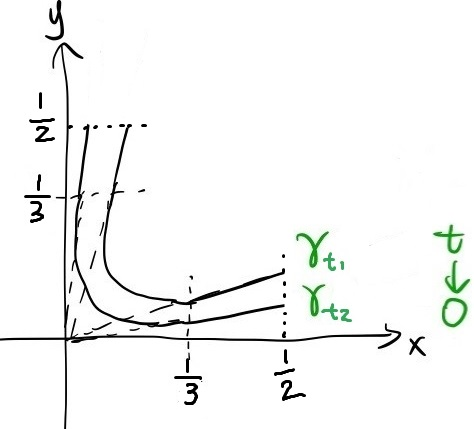
\includegraphics[scale=0.3]{gamma_t.jpg}
%\end{figure}

satisfying the following conditions: 
\begin{itemize}
\item 
$\gamma:(0,\rho)\times[-1/2,1/2]\to\R^2$,defined by $\gamma(t,s)=\gamma_t(s)$ is a smooth embedding, and its image lies in the ($x>0,y>0$) quarter of $\R^2$;
\item for $s\leq-1/3$, $\gamma_t(s)=(-ts,-s)$; 
\item for $s\geq1/3$, $\gamma_t(s)=(s,ts)$;  
\item for all $s\in[-1/2,0]$, $\lim_{t\to0}\gamma_t(s)=(0,-s)$;
\item for all $s\in[0,1/2]$, $\lim_{t\to0}\gamma_t(s)=(s,0)$. 
\end{itemize}

We can now define $E_\rI|_{S^{d-1}\times[-\frac{1}{2},\frac{1}{2}]\times B_1\times B_2\times(0,\rho)}$.

Take the trivial bundle 
$\R^d\times S^{d-1}\times[-\frac{1}{2},\frac{1}{2}]\times B_1\times B_2\times(0,\rho)$. 
For a constant $1\le c\le2$, let $Z_1(c)$ (resp. $Z_2(c)$) be the disk sub-bundle of this trivial bundle whose fiber over $$b=(\theta,\eta,b_1,b_2,t)\in S^{d-1}\times[-\frac{1}{2},\frac{1}{2}]\times B_1\times B_2\times(0,\rho)$$ 
is $\D_{p_1}(cx)$ (resp. $\D_{p_2}(cy)$), 
where $p_1,p_2\in\R^d$ are such that \begin{equation}\label{xyp1p2_eqn}
|p_2-p_1|=1, \frac{p_2-p_1}{|p_2-p_1|}=\theta, p_1+p_2=0; \tn{ and } (x,y)=\gamma_t(\eta).
\end{equation}

For $i=1,2$ and $1\le c\le2$, we also define the pull-back bundle 
\[\begin{tikzcd}
(\pr^2_{B_i})^*E_i(c)\rar\dar & E_i(c)\dar["\pi_i"]\\
S^{d-1}\times[-\frac{1}{2},\frac{1}{2}]\times B_1\times B_2\times(0,\rho)\rar["\pr^2_{B_i}"] & B_i
\end{tikzcd}
\]
where $\pr^2_{B_i}$ is the projection to the $B_i$ factor. 

Now, define $E_\rI|_{S^{d-1}\times[-\frac{1}{2},\frac{1}{2}]\times B_1\times B_2}$ by removing $Z_1(1)$ and $Z_2(1)$ from the trivial bundle $\R^d\times S^{d-1}\times[-\frac{1}{2},\frac{1}{2}]\times B_1\times B_2$ 
and glue back $(\pr^2_{B_1})^*E_1(2)$ and $(\pr^2_{B_2})^*E_2(2)$, respectively, via the following diffeomorphisms that preserves framing up to scaling by a constant: 
$$Z_1(2)-Z_1(1)\stackrel{\tau'_1}{\approx} (\pr^2_{B_1})^*E_1(2)-(\pr^2_{B_1})^*E_1(1),\qquad Z_2(2)-Z_2(1)\stackrel{\tau'_2}{\approx} (\pr^2_{B_2})^*E_2(2)-(\pr^2_{B_2})^*E_2(1).$$

It is easy to see that, over the overlapping parts of the there pieces (\ref{piecesB_eqn}) of the base, the definitions in Section \ref{first_subsubsec} and in Section \ref{second_subsubsec} agree, after we properly scale and translate $\R^d$. 

This completes the definition of $\pi_\rI:E_\rI\to E_\rI$. 
Note that we clearly have a ``section at $\infty$'', 
$$\sigma_\rI:B_\rI\longrightarrow E_\rI$$
induced from $\sigma_1$ and $\sigma_2$. 
And $\pi_\rI$ is an $(M_1\#M_2,\infty)$-bundle, where $\#$ denotes connect sum. 


\subsection{Specifying an induced framing on the bracket bundle}

On fibers over $S^{d-1}\times[-\frac{1}{2},\frac{1}{2}]\times B_1\times B_2\times(0,\rho)$ it is the obvious one. 

Next, we specify a vertical framing $F_\rI$ on $E_\rI|_{E_1(3)^\circ\times B_2\times (0,\rho)}$. 
(The $E_\rI|_{B_1\times E_2(3)^\circ\times (0,\rho)}$ case is similar, so we omit it below.)
Recall that when defining $E_\rI|_{E_1(3)^\circ\times B_2\times (0,\rho)}$, we remove $\cN(s_1,t)$ from $(\pr^1_{B_1})^*E_1$ and glue back $(\pr^1_{B_2})^*E_2(\rho_0/t)$ using the diffeomorphism (\ref{filling_eqn}): 
\begin{align*}
(\pr^1_{B_2})^*E_2(\rho_0/t)-(\pr^1_{B_2})^*E_2(1)\stackrel{\tau'_2}{\approx}(\D^d(\rho_0/t)-\D^d(1))\times E_1(3)\times B_2\times(0,\rho) \nonumber\\
\stackrel{\tn{scaling by }t}{\approx}\mathcal{D}(\rho_0)-\mathcal{D}(t)\stackrel{\exp}{\approx}\cN(s_1,\rho_0)-\cN(s_1,t).
\end{align*}
%Equivalently, for any $1<N<\rho_0/t$ we can glue back $\tilde{E}'_2(N)$ via the diffeomorphism
%$$\tilde{E}'_2(N)-\tilde{E}'_2(1)\stackrel{\tau'_2}{\approx}(\D^d(N)-\D^d(1))\times E_1(3)\times B_2\times(0,\rho)\stackrel{\tn{scaling}}{\approx}\cN(s_1,N)-\cN(s_1,1).$$
Now, 
\begin{itemize}
\item On $(\pr^1_{B_1})^*E_1-\cN(s_1,2\sqrt{t})$, let $F_\rI$ be $f_1^*F_1$. (Note that since $t<\rho$, $2\sqrt{t}<\rho_0$.)
\item On $(\pr^1_{B_2})^*E_2(1/\sqrt{t})$, let $F_\rI$ be $(f'_2)^*F_2$. (Note that since $\rho<1$, $1/\sqrt{t}>1$.)
\item It remains to specify $F_\rI$ on the region
\begin{equation}\label{annulus_eqn}
(\pr^1_{B_2})^*E_2(2/\sqrt{t})-(\pr^1_{B_2})^*E_2(1/\sqrt{t})\stackrel{(\ref{filling_eqn})}{\approx}\cN(s_1,2\sqrt{t})-\cN(s_1,\sqrt{t}).
\end{equation}
Since the diffeomorphism (\ref{filling_eqn}) is not framing-preserving, we need to choose a homotopy in-between. 
The existence of such a homotopy is clear. So we choose and fix a framing on the region (\ref{annulus_eqn}), that smoothly extends $F_\rI$ on the parts it has already been defined; and define $F_\rI$ on the region (\ref{annulus_eqn}) using this framing we chose. 
\end{itemize}

Now that $F_\rI$ is defined, for $p\in E_\rI$, we define  $\exp_p$, $\tn{radius}^{\max}(p)$, $D_p(\epsilon)$ in the same way as in Section \ref{notation11_sec}. 

\subsection{Defining the compactified base of the family of bracket bundles}
%and \cmt{or not} the universal family (the $[0,\rho)$-parameterized bracket bundle) over it}

%\subsubsection{Defining the base $B_I$}
In this section, we define $B_I$, the compactified base of the family of bracket bundles. 
The space $B_I$ is a compactification of 
$B'\times(0,\rho)$ on the 0 side. More precisely, it is obtained by gluing together the following 3 pieces: 
\begin{equation}\label{piecesBtl_eqn}
E_1(3)^\circ\times B_2\times[0,\rho),\quad S^{d-1}\times L\times B_1\times B_2,\quad B_1\times E_2(3)^\circ\times[0,\rho),
\end{equation}
where $L\subset \R^{\ge0}\times\R^{\ge0}$ is the $L$-shaped region enclosed by the blue lines below. (The solid blue lines are within $L$ and the dashed blue curve is not in $L$ but just part of the boundary of $L$.)

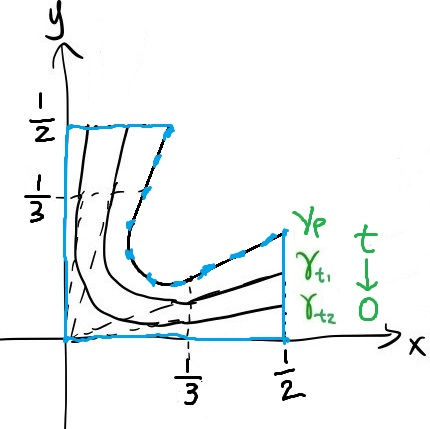
\includegraphics[scale=0.3]{gamma.jpg}

We have a homeomorphism (if we define $\gamma_0$ in the obvious way -- it goes along the left and bottom blue lines, from $(0,1/2)$ to $(1/2,0)$)
\begin{align}\label{L_eqn}
[-\frac{1}{2},\frac{1}{2}]\times[0,\rho)&\longrightarrow L\\
(s,t)&\longrightarrow \gamma_t(s),\nonumber
\end{align}
which is a diffeomorphism except at the point $(0,0)\in L$. 

With the identification (\ref{L_eqn}), we define $B_I$ by gluing the 3 pieces in (\ref{piecesBtl_eqn}), in the exact same way as how we defined $B'$ in Section \ref{Bt_sec}, but now with everything timed with $[0,\rho)$. 
The result is a manifold with boundary and corners. 
The main stratum is $B_\rI$. 
It has 2 codim-1 boundary strata: 
\begin{itemize}
\item one is by gluing together $E_1(3)^\circ\times B_2\times\{0\}$ and $S^{d-1}\times(-\frac{1}{2},0)\times\{0\}\times B_1\times B_2$ above; we call this stratum $BS^+$;
\item the other is by gluing together $B_1\times E_2(2)^\circ\times\{0\}$ and $S^{d-1}\times(0,\frac{1}{2})\times\{0\}\times B_1\times B_2$ above; we call this stratum $BS^-$.
\end{itemize}
And it has 1 codim-2 corner stratum which we call $BS'$:
\begin{itemize}
\item $BS'=S^{d-1}\times\{0\}\times\{0\}\times B_1\times B_2$, a subset of the second piece in (\ref{piecesBtl_eqn}). 
\end{itemize}

Below is a picture of $B_I$ when $d=2$, $B_1=B_2=$point, with its map to $[0,\rho)$. Here $B_I$ is visualized as a family of spheres parameterized by $[0,\rho)$ (in the picture, the sphere with bigger parameter is more inside). The outside most one (the one parameterized by $0$), is actually not a smooth sphere---the upper and lower hemispheres are not glued together in a smooth way. 

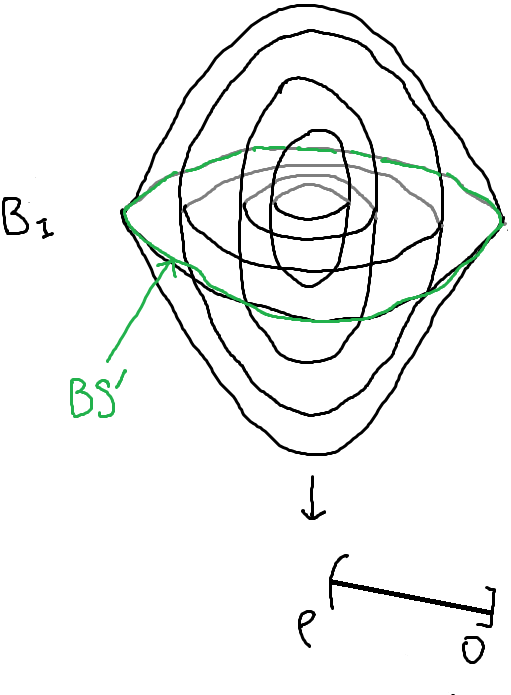
\includegraphics[scale=0.5]{BI_fig} 


In Section \ref{conftilde_sec} later, we will define, for a finite set $A$, $\wt{C}_A$ \cmt{what I called $\wt{Conf}_A$ in the emails}---the ``family'' configuration space. 
$\wt{C}_\emptyset$ is just $B_I$ here. 



$B_I$ should be thought of a the parameter space of the fibers of bracket bundles (with different smoothing parameter $t\in[0,\rho)$). A picture of what the points of $B_I$ are parameterizing:

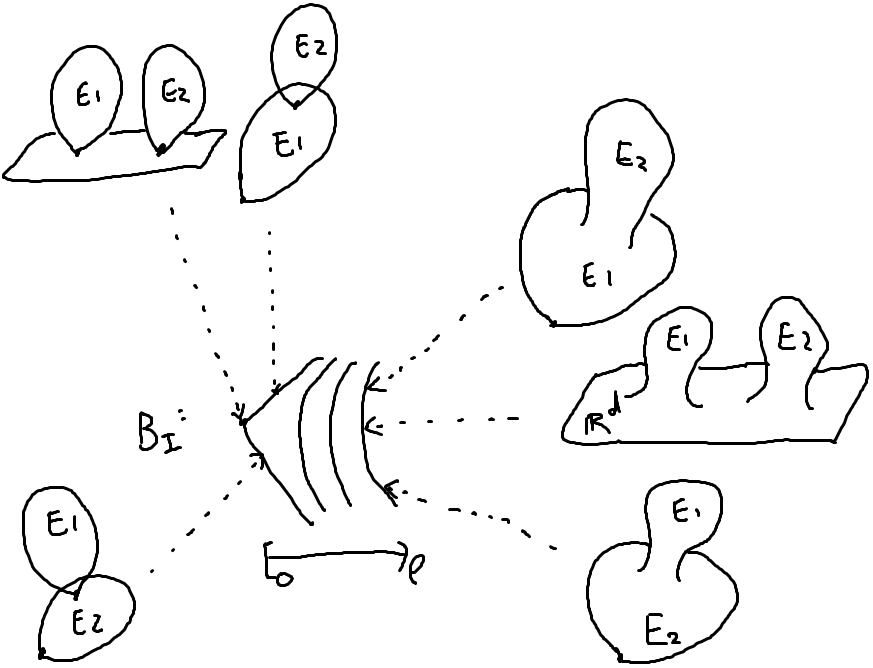
\includegraphics[scale=0.5]{EI_fig} 

We can't quite make this statement rigorous by defining a smooth ``universal family'' over $B_I$, because it will have singularities along the nodes. 



%\subsubsection{Defining the (singular) total space? \cmt{may not be necessary}}
%
%\cmt{This section is largely not yet completed}
%
%In this section we define a topological space, $E_I$, with a map $\pi_I:E_I\to B_I$. Intuitively, $E_I$ is the ``universal family'' of bracket bundles parameterized by $B_I$. 
%A picture of some fibers of $\pi_I$: 
%
%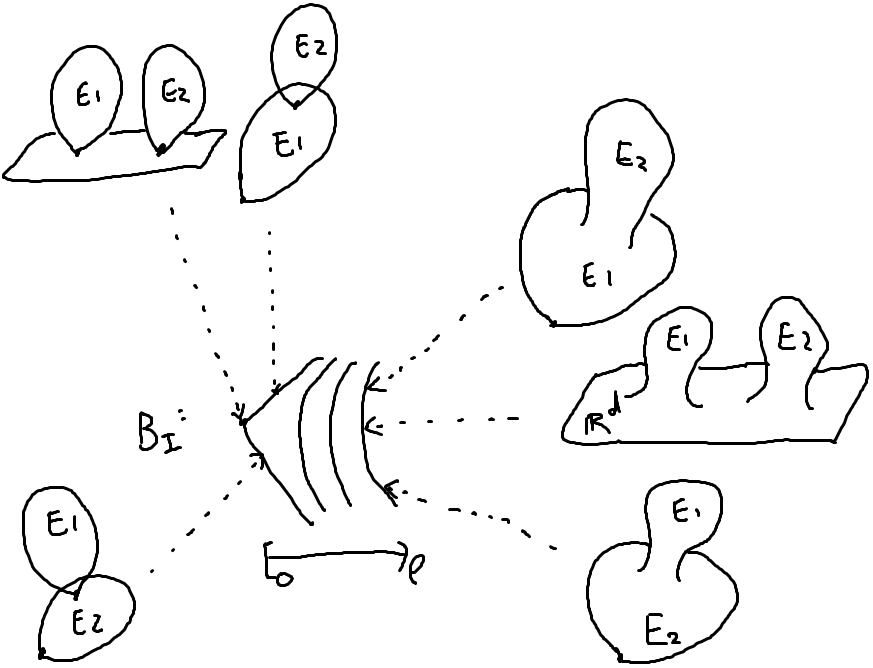
\includegraphics[scale=0.5]{EI_fig}
%
%If we remove the part of $E_I$ where the nodes lie, then it becomes a smooth manifold and $\pi_I$ becomes a submersion.
%With the part where the nodes lie, $E_I$ is singular.  
%
%First, we define $E_I$ over each stratum of $B_I$. 
%\begin{itemize}
%\item Over the main stratum $B_\rI$: $E_I|_{B_\rI}$ is just $E_\rI$. 
%\item Over $BS^+$: define $(\pr^1_{B_1})^*E_1\to E_1(3)\times B_2\times\{0\}$ and $s_1:E_1(3)\times B_2\times\{0\}\to(\pr^1_{B_1})^*E_1$ in the same way as at the beginning of Section \ref{first_subsubsec}, but with $(0,\rho)$ replaced with $\{0\}$. Define $E_I|_{BS^+}=$
%\end{itemize}





\subsection{Specifying a ``trivialization near infinity'' on the bracket bundle}
\label{tauEI_subsec}

In this section we specify a trivialization 
$$\tau_\rI: U_\rI\longrightarrow B_\rI\times(\R^d\backslash\D^d(3))$$
of $E_\rI-\sigma_\rI(B_\rI)$ in some neighborhood $U_\rI$ or $\sigma_\rI(B_\rI)$. 
%, for some function $g: B_\rI\to\R^{\ge1}$. 
Once this is done, we define, for $N\ge3$, 
$$E_\rI(N)=E_\rI-\Big((\tau_\rI)^{-1}\big(B_\rI\times(\R^d\backslash\D^d(N))\big)\Big),\qquad E_\rI(N)^\circ=E_\rI-\Big((\tau_\rI)^{-1}\big(B_\rI\times(\R^d\backslash\mr\D^d(N))\big)\Big).$$

%$g':B_\rI\to\R^{\ge1}$, $g'\ge g$, 
%$$E_\rI(g')=E_\rI-\Big((\tau_\rI)^{-1}(\mr\cA_{\pi_\rI}(g'))\Big),\qquad E_\rI(g')^\circ=E_\rI-\Big((\tau_\rI)^{-1}(\cA_{\pi_\rI}(g'))\Big).$$


\subsubsection{when one bundle is inside another, trivialization near infinity of the bigger bundle}
\label{trivEI1_subsubsec}
As before, for $i=1,2$, define the tautological bundle 
$$\pi_i^*E_i\xrightarrow{\pi_i^*\pi_i}E_i-\sigma_1(B_i)$$
as the pull-back
\[
\begin{tikzcd}
\pi_i^*E_i \rar["f_i"] \dar["\pi_i^*\pi_i"] & E_i\dar["\pi_i"] \\
E_i-\sigma_i(B_i)\rar["\pi_i"] & B_i,
\end{tikzcd}
\]
and define 
$$s_i:E_i-\sigma_i(B_i)\to\pi_i^*E_i,\qquad s_i(p)=f_i^{-1}(p)$$
its canonical section. 
Recall we have specified trivializations 
$$\tau'_i:U'_i=E_i-\sigma_i(B_i)-E_i(1)\xrightarrow{\approx} B_i\times (\R^d\backslash\D^d).$$
Write $\tau^{\R^d}_i:E_i-\sigma_i(B_i)-E_i(1)\to\R^d\backslash\D^d$ the composition of $\tau'_i$ with the projection to the $\R^d\backslash\D^d$ factor. 


Now, we specify a trivialization 
$$\hat\tau'_i:\hat{U}'_i\longrightarrow
\big(E_i-\sigma_i(B_i)\big)\times\big(\R^d\backslash\D^d(3)\big)$$
of $\pi_i^*\pi_i$ in a (center-removed) neighborhood $\hat{U}'_i$ of the pulled-back section $\pi_i^*\sigma_i$. Before spelling out the details, what we want to do is the following: 
\begin{itemize}
\item On fibers over $E_i(2)$, $\hat\tau'_i$ is just the pull-back $\pi_i^*\tau'_i$. 
\item On a fiber over $p\in E_i-\sigma_i(B_i)-E_i(3)$, $\hat\tau'_i$ is defined as follows. 
\begin{itemize}
\item First, shifting $\pi_i^*\tau'_i$, via a translation in $\R^d$, so that the ``center'' becomes the point ``$1/2p$''. 
Here is an illustration: 

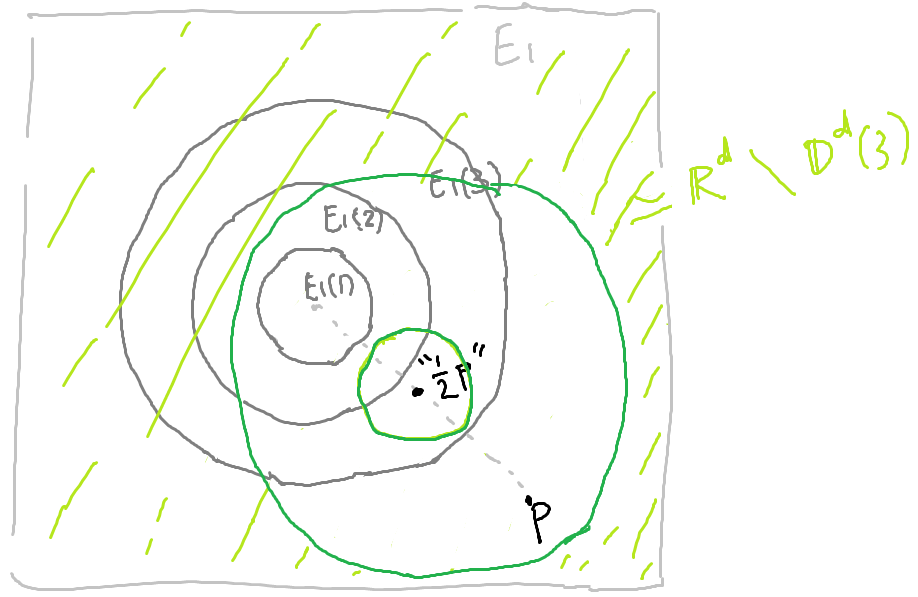
\includegraphics[scale=0.5]{trivbrak1_fig}

In this picture, the spheres centered at 0 in $\R^d$, under $\pi_i^*\tau'_i$, are the gray circles; the light-green identification represents $\hat\tau'_i$. 
\item Next, as $p$ goes further away from $E_i(3)$, we also re-scale so that, 
although the radius of $(\hat{U}'_i)|_p$ gets bigger and bigger (because $(\hat{U}'_i)|_p$ cannot intersect $f_i^{-1}(E_i(1))$), with respect to $\pi_i^*\tau'_i$, 
we want the radius of $(\hat{U}'_i)|_p$ to stay constant with respect to $\hat\tau'_i$.  
\end{itemize}
\item Over $E_i(3)-E_i(2)$, we gradually increases the shifting from 0 (the first case above) to shifting by $\frac{1}{2}p$ (the second case above). 
\end{itemize}

Once $\hat\tau'_i$ is defined, we denote 
$$\hat{E}_i(N)=\pi_i^*E_i-\Big((\hat\tau'_i)^{-1}\big((E_i-\sigma_i(B_i))\times\R^d\backslash\D^d(N)\big)\Big).$$


\cmt{The rest of Section \ref{tauEI_subsec} can be skipped when first reading.}

The details of defining $\hat\tau'_i$ is as follows:

First, define a smooth function
$g_i:E_i-\sigma_i(B_i)\to \R^{\ge1}$ by: 
when $p\in E_i(2)$, 
$g_i(p)=
3$; when $p\in E_i-\sigma_i(B_i)-E_i(3)$, 
$g_i(p)= 3|\tau^{\R^d}_i(p)|$; 
when $p\in E_i(3)-E_i(2)$, $g_i$ is an arbitrarily chosen increasing function that makes $g_i(p)$ smooth. 

\begin{itemize}
\item Over $E_i(2)$, define $\hat{U}'_i=f_i^{-1}(E_i-\sigma_i(B_i)-E_i(3))$ and $\hat\tau'_i=\pi_i^*\tau'_i|_{E_i-\sigma_i(B_i)-E_i(3)}$. 
\item Over $E_i-\sigma_i(B_i)-E_i(3)$, define $\hat{U}'_i\subset \pi^*_iE_i$ such that, for $p\in E_i-\sigma_i(B_i)-E_i(3)$, 
$$\hat{U}'_i\cap (\pi_i^*\pi_i)^{-1}(p)=f_i^{-1}\Big(E_i|_{\pi_i(p)}-\sigma_i(B_i)-E_i(1)-(\tau^{\R^d}_i)^{-1}\big(\D^d_{\frac{1}{2}\tau^{\R^d}_i(p)}(g_i(p))\backslash\D^d\big)\Big)$$
and, for $\tilde{p}\in \hat{U}'_i\cap(\pi_i^*\pi_i)^{-1}(p)$, 
$$\hat\tau'_i(\tilde{p})=\Big(p,\ 
\frac{3}{g_i(p)}\cdot\big(\tau^{\R^d}_i\big(f_i(\tilde p)\big)-\frac{1}{2}\tau^{\R^d}_i(p)\big)\Big)\in  \big(E_i-\sigma_i(B_i)\big)\times \R^d\backslash\D^d(3).$$
\item Over $E_i(3)-E_i(2)$: let $\lambda:[2,3]\to[0,1/2]$ be a smooth monotonically increasing function such that $\lambda'(0)-\lambda'(1)=0$; given $p\in E_i(3)-E_i(2)$, define $p'=\lambda(|\tau^{\R^d}_i(p)|)\cdot\tau^{\R^d}_i(p)\in\R^d$; 
then, for $p\in E_i(3)-E_i(2)$, define
$$\hat{U}'_i\cap (\pi_i^*\pi_i)^{-1}(p)=f_i^{-1}\Big(E_i|_{\pi_i(p)}-\sigma_i(B_i)-E_i(1)-(\tau^{\R^d}_i)^{-1}\big(\D^d_{p'}(g_i(p))\backslash\D^d\big)\Big)$$
and, for $\tilde{p}\in \hat{U}'_i\cap(\pi_i^*\pi_i)^{-1}(p)$, 
$$\hat\tau'_i(\tilde{p})=\Big(p,\ \frac{3}{g_i(p)}\cdot\big(\tau^{\R^d}_i\big(f_i(\tilde p)\big)-p'\big)\Big).$$
\end{itemize}

Now that we have defined $\hat\tau'_1$ (resp. $\hat\tau'_2$), by simply taking a product with $B_2\times(0,\rho)$ (resp. $B_1\times(0,\rho)$), it induces a trivialization of 
\begin{align*}
(\pr^1_{B_1})^*E_1&\xrightarrow{(\pr^1_{B_1})^*(\pi_1)}E_1(3)^\circ\times B_2\times(0,\rho)\\
\big(\tn{resp. }\qquad (\pr^2_{B_2})^*E_2&\xrightarrow{(\pr^2_{B_2})^*(\pi_2)}B_1\times E_2(3)^\circ\times(0,\rho)\qquad\big)
\end{align*}
near $(\pr^1_{B_1})^*\sigma_1(B_1)$ (resp. $(\pr^2_{B_2})^*\sigma_2(B_2)$).
Since the construction of $E_\rI$ over $E_1(3)^\circ\times B_2\times(0,\rho)$ and $B_1\times E_2(3)\times(0,\rho)$ is done by doing some surgery on $(\pr^1_{B_1})^*E_1$ and $(\pr^2_{B_2})^*E_2$, $\hat\tau'_1$ induces a trivialization of $E_\rI|_{E_1(3)^\circ\times B_2\times(0,\rho)\cup B_1\times E_2(3)^\circ\times(0,\rho)}$ near $\sigma_\rI(B_\rI)$. 

\subsubsection{Trivialization of the bracket bundle near infinity}

Recall that $E_\rI$ is defined by gluing the 3 pieces
$$E_\rI|_{E_1(3)^\circ\times B_2\times(0,\rho)},\qquad E_\rI|_{S^{d-1}\times(-\frac{1}{2},\frac{1}{2})\times B_1\times B_2\times (0,\rho)},\qquad E_\rI|_{B_1\times E_2(3)^\circ\times(0,\rho)}$$
together. 
We want to define a trivialization $\tau_\rI$ of $E_\rI$ near $\sigma_\rI$.
On the first and third part of $E_\rI$ above, let $\tau_\rI$ be given as in Section \ref{trivEI1_subsubsec}. 
It remains to define $\tau_\rI$ on the second part of $E_\rI$. 
Over $S^{d-1}\times\big((-\frac{1}{2},-\frac{1}{3})\cup(\frac{1}{3},\frac{1}{2})\big)\times B_1\times B_2\times (0,\rho)$, it coincides with the definition of $\tau_\rI$ on the other two pieces, via gluing. 
Over $S^{d-1}\times[-\frac{1}{3},\frac{1}{3}]\times B_1\times B_2\times (0,\rho)$, 
we define $\tau_\rI$ to be given by the standard trivialization on the trivial bundle $\R^d\times S^{d-1}\times[-\frac{1}{3},\frac{1}{3}]\times B_1\times B_2\times (0,\rho)$, from which $E_\rI|_{S^{d-1}\times[-\frac{1}{2},\frac{1}{2}]\times B_1\times B_2\times (0,\rho)}$ is obtained by surgery. 
Note that, by (\ref{xyp1p2_eqn}), this means the mid-point of the centers of the two disks to be removed when performing this surgery is 0 under this trivialization. 
The definition in Section \ref{trivEI1_subsubsec} ensures that the $\tau_\rI$ defined this way is smooth. 

\section{The Strata of  \texorpdfstring{$\wt{C}_A$}{the big configuration space}}

For a finite set $S$, denote by $|S|$ the number of elements in $S$. 

Let $A$ be a finite set. 
In this section we describe the strata of $\wt{C}_A$. 

\subsection{The combinatorics}
\begin{dfn}An {\it $A$-labeled tree} consists of
\begin{itemize}
\item a tree $T$---we denote by $V(T), E(T)$ the vertex and edge set of $T$, respectively;
\item $r\in V(T)$, ``the root''; 

for two vertices $v\neq w\in V(T)$, if the unique path between $v$ and $r$ passes through $w$, we say $w$ is an {\it ancestor} $v$ and $v$ is a {\it descendant} of $w$, and denote $v>w$; 
if, additionally, $v$ and $w$ are also adjacent, then we say $w$ is the {\it parent} of $v$ and $v$ is a {\it child} of $w$;  

denote the set of children of $v$ by $cld(v)$; 

for an edge $e\in E(T)$, say the vertex adjacent to $e$ and closer to $r$ {\it just below} $e$, denoted by $v_-(e)$ and the vertex adjacent to $e$ and further away from $r$ {\it just above} $e$, denoted by $v_+(e)$; 

\item every vertex $v\in V(T)$ is associated with one of the four labels: $\R^d, \pi_1, \pi_2,\pi_\rI$; call it the ``space label'', denoted by $ls(v)$; 

\item every vertex $v\in V(T)$ is associated with a subset of $A$; call it the ``points label'', denoted by $lp(v)$;
\end{itemize}
satisfying the following conditions
\begin{itemize}
\item either 

both $\pi_1, \pi_2$ are associated to exactly one vertex, and no vertex is associated to $\pi_\rI$;

or

$\pi_\rI$ is associated to exactly one vertex, and no vertex is associated to $\pi_1$ or $\pi_2$; 
\item if $v\neq w \in V(T)$, then $lp(v)\cap lp(w)=\emptyset$;
\item $\bigsqcup_{v\in V(T)}lp(v)=A$;
\item if $v\in V(T)$ is such that $ls(v)=\R^d$, then $|cld(v)|+|lp(v)|\ge2$. 
\end{itemize}
\end{dfn}

\begin{dfn}
For notational convenience, define $\ov{cld}(v)=cld(v)\sqcup lp(v)$. 
\end{dfn}

\begin{minipage}{.6\textwidth}
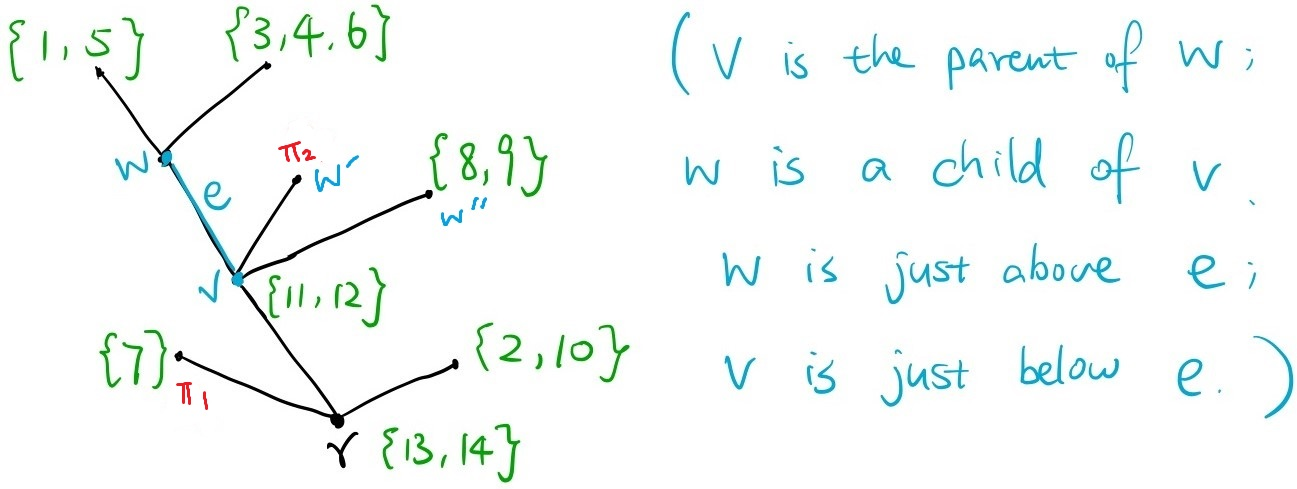
\includegraphics[scale=0.2]{tree_fig}
\end{minipage}
\begin{minipage}{.4\textwidth}
(In this example, $A=\{1,2,\ldots,14\}$; the point labels are green and space labels are red. When a space label is $\R^d$, it is omitted.)
\end{minipage}


Denote by $\cT(A)$ the set of $A$-labeled trees. 
The strata of $\wt{C}_A$ will be labeled by elements of $\cT(A)$. 
Note that the conditions above implies that, if $T\in\cT(A)$ has only one vertex, then its space label must be $\pi_\rI$ and its points label must be $A$. 

\begin{dfn}
We define an ``addition'' operation on the set of space labels $\{\R^d,\pi_1,\pi_2,\pi_\rI\}$: 
first define a map ($\mathcal{P}$ means power set)
\begin{align}
\tn{lsset}:\{\R^d,\pi_1,\pi_2,\pi_\rI\}&\longrightarrow \mathcal{P}\{1,2\}\\
\R^d\to\emptyset,\qquad \pi_i&\to \{i\},\qquad \pi_\rI\to\{1,2\}\nonumber.
\end{align}
Then, for $X,Y\in \{\R^d,\pi_1,\pi_2,\pi_\rI\}$, define $X+Y=\tn{lsset}^{-1}(\tn{lsset}(X)\cup\tn{lsset}(Y))$. 
\end{dfn}

\begin{dfn}
For $T\in\cT(A)$, let $T/e\in\cT(A)$ be the tree obtained by contracting $e$---merging the two vertices connected to $e$ into a single vertex, taking a union of their point labels and sum (in the sense above) of their space labels. 
Similarly, if $I\subset E(T)$, denote by $T/I\in\cT(A)$ the tree obtained by contracting all edges in $I$. 

%use the following rule to determine the new vertex's space label from old vertices' space labels: 
%
%\begin{tabular}{c | c | c | c}
%space label of the old vertices & $\R^d$ and $X$ ($X=\R^d$ or $E_1$ or $E_2$ or $E_\rI$) & $E_1$ and $E_2$ \\ \hline
%space label of the new vertex & $X$ & $E_\rI$
%\end{tabular}

We denote the new vertex in $V(T/e)$ by $[e]$. 
From the definition of $T/e$, there are obvious maps 
$$\tn{contr}^V_{T;e}:V(T)\longrightarrow V(T/e)$$
which maps $v_-(e),v_+(e)$ to $[e]$ and every other vertex to itself, and
$$\tn{contr}^E_{T;e}:E(T)\backslash\{e\}\longrightarrow E(T/e)$$
which maps every edge to itself. 
\end{dfn}

\subsection{Describing each stratum}
\label{stratum2_sec}

Let $T$ be an $A$-labeled tree. 
For $v\in V(T)$, define  
$$\tn{Space}(v)=C_{\ov{cld}(v)}(ls(v));$$
i.e., the (uncompactified) configuration space of $\ov{cld}(v)$-labeled points in $ls(v)$. 
For example, for the vertex $v$ in the picture above, $$ls(v)=\R^d, lp(v)=\{11,12\}, cld(v)=\{w,w',w''\},$$
so $\tn{Space}(v)=C_{\{11,12,w,w',w''\}}(\R^d)$. 

Define $S_T=\prod_{v\in V(T)}\tn{Space}(v)$. 
In particular, when $T$ has only one vertex, $S_T=C_A(\pi_\rI)$. 
It follows from definition that $S_T$ is a smooth manifold; it is also the total space of a smooth fiber bundle over $B_1\times B_2$. 

{\it Example:} if $A=\{1,2,3,4\}$ and $T$ is the tree below on the left, then $S_T$ consists of configurations like the picture below on the right. 

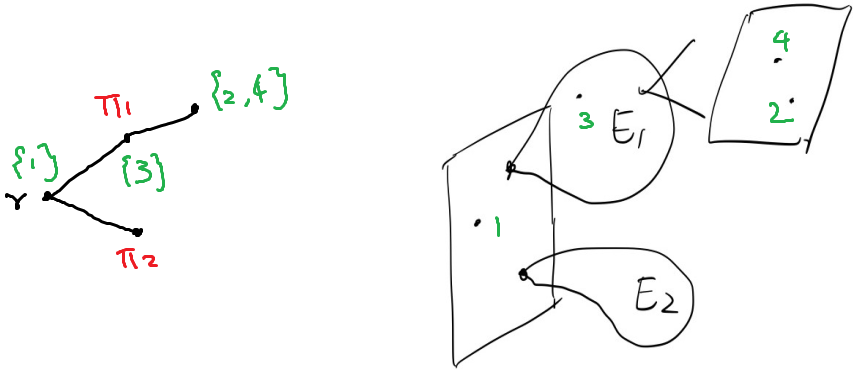
\includegraphics[scale=0.5]{ST_fig}

Define $\wt{C}_A=\bigsqcup_{T\in\cT(A)}S_T$ as a set. 

\subsection{More notation; normalization}
\label{normalization_subsec}
%Suppose $A$ admits a total order. 

Given $T\in\cT(A)$ and $v\in V(T)$, define
$$lp(\ge v)=\{a\in A\big|\,\exists v'\in V(T),v'\ge v, a\in lp(v')\}$$
and 
$$ls(> v)=\{x\in\{\pi_1,\pi_2\}\big|\, \exists v'\in V(T), v'>v, \tn{lsset}(x)\subset\tn{lsset}(ls(v'))\}.$$
%ls(v')=x\tn{ or }\pi_\rI\}.$$
We then define a ``forgetful map'' 
\begin{align*}
f_v:lp(\ge v)\sqcup ls(>v)&\longrightarrow \ov{cld}(v)\\
f_v(x)=&\begin{cases}x, \tn{ if }x\in lp(v);\\ w\in cld(v) \tn{ such that }\exists v'\ge w, x\in lp(v') \tn{ or }\tn{lsset}(x)\subset\tn{lsset}(ls(v')), \tn{ otherwise}.\end{cases}
\end{align*}
For example, if $T$ is as in the example in Section \ref{stratum2_sec}, then 
$$f_r(2)=f_r(4)=f_r(3)=f_r(\pi_1)=\tn{the vertex carrying }\pi_1 \tn{ and } 3\in cld(r).$$



%\begin{dfn}
%Suppose $x=(x_v)_{v\in V(T)}\in S_T=\prod_{v\in V(T)}\tn{Space}(v)$ and $v\in V(T)$ is such that $ls(v)=\R^d$. 
%We first define a (very artificial) total order on $ls(>v)\sqcup lp(\ge v)$ by requiring: 
%\begin{itemize}
%\item all elements in $ls(>v)$ are smaller than elements in $lp(\ge v)$; 
%\item $E_1<E_2$ if both are in $ls(>v)$; 
%\item elements in $lp(\ge v)$ are ordered the same as in $A$. 
%\end{itemize}
Suppose $x=(x_v)_{v\in V(T)}\in S_T=\prod_{v\in V(T)}\tn{Space}(v)$ and $v\in V(T)$ is such that $ls(v)=\R^d$. 

\begin{dfn}
The {\it weight} of an element $n\in \ov{cld}(v)$ is 
$$\begin{cases}
1,\tn{ if }n\in lp(v)\\
%\tn{number of elements in }
|f_v^{-1}(n)|, \tn{ if }n\in cld(v) \tn{ and } f_v^{-1}(n)\cap ls(>v)=\emptyset\\
\infty, \tn{ if }f_v^{-1}(n)\cap ls(>v)\neq\emptyset.
\end{cases}$$
\end{dfn}
For example, if $x$ and $v$ are like this 

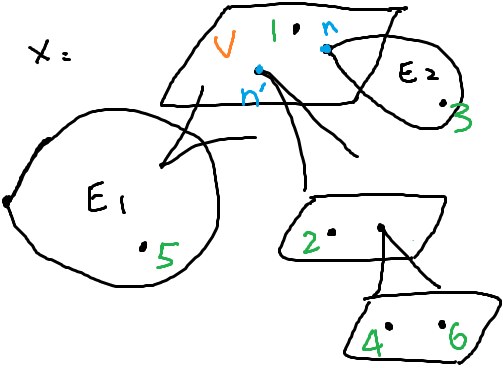
\includegraphics[scale=0.5]{ST2_fig}

then, on the $v$-screen, the marked point 1 has weight 1, the node $n$ has weight $\infty$, and the node $n'$ has weight 3.

\begin{dfn}\label{screennormalize_dfn}
Suppose $i,j\in \ov{cld}(v), i\neq j$. 
We define a {\it standard representative (depending on $i,j$)}, $x'_v\in (\R^d)^{\ov{cld}(v)}$, 
in the equivalence class $x_v\in C_{\ov{cld}(v)}(\R^d)$ (recall the equivalence relation here is modulo translation and scaling of $\R^d$):
$x'_v$ is such that 
\begin{itemize}
\item $0\in\R^d$ is located at the ``center of gravity'' of points in $\ov{cld}(v)$ (for example, in the picture above, the center of gravity of the $v$-screen coincides with the node $n$); note there is a bit of ambiguity: in the case there are 2 elements in $\ov{cld}(v)$ with weight $\infty$, we define the center of gravity to be the mid-point of these two elements; 

\item the scaling is such that the distance between the points $i$ and $j$ is 1. 
\end{itemize}
\end{dfn}

For each $T\in \cT(A)$ and $v\in V(T)$, we choose, arbitrarily, $i\neq j\in \ov{cld}(v)$, and fix these choices for the rest of the document. 
We can therefore talk about the standard representative $x'_v$ of $x_v$. 

In Section \ref{conftilde_sec}, we will define a smooth manifold structure on $\wt{C}_A$ by ``smoothing out the nodes''. To prepare for this, we next define the largest and smallest radii on each screen where the smoothing can take place. 

\begin{dfn}\label{Rmin_dfn}
Suppose $x=(x_v)_{v\in V(T)}\in S_T$, $v\in V(T)$. 
%, and $i\neq j\in \ov{cld}(v)$. 
Define $R^{\min}(x;v)$ as follows: 
\begin{itemize}
\item if $ls(v)=\R^d$, then $R^{\min}(x;v)=$
$$2\cdot\inf\{R\in\R^{\ge1}\big|\,\tn{in the configuration }x'_v,\tn{ all marked points and nodes are inside }\D^d(R)\};$$
\item if $ls(v)=\pi_i$, $i=1$ or 2 or $\mr{I}$, and $ls(>v)=\emptyset$, 
then $R^{\min}(x;v)=$
$$2\cdot\inf\{R\in\R^{\ge1}\big|\,\tn{in the configuration }x_v,\tn{ all marked points and nodes are inside }E_i(R)\};$$
\item if $ls(v)=\pi_i$, $i=1$ or 2, and $ls(>v)=\{\pi_{3-i}\}$: denote by $\star_v\in E_i-\sigma_i(B_i)$ the position of the marked point $f_v(\pi_{3-i})$ in the configuration $x_v$, then we can view $x_v$ as an element in 
$$C_{\ov{cld}(v)\backslash\{f_v(E_{3-i})\}}(\pi_i^*E_i)|_{\star_v},$$
where $\pi_i^*E_i$ is the total space of 
%$\pi_i^*\pi_i:\pi_i^*E_i\to E_i-\sigma_i(B_i)$ 
the tautological bundle as in Section \ref{trivEI1_subsubsec}, and $(\pi_i^*E_i)|_{\star_v}$ denotes the fiber of $\pi_i^*(E_i)$ over the point $\star_v$;
now define $R^{\min}(x;v)=$
$$2\cdot\inf\{R\in\R^{\ge3}\big|\,\tn{in the configuration }x_v,\tn{ all marked points and nodes are inside }\hat E_i(R)\}.$$
\end{itemize}
\end{dfn}

\begin{dfn}\label{rmax_dfn}
Suppose $x=(x_v)_{v\in V(T)}\in S_T$, and $e\in E(T)$. Note that $v_+(e)\in cld(v_-(e))$. If $ls(v_-(e))\neq\R^d$, we denote by $\star_e\in ls(v_-(e))$ the location of the $v_+(e)$-marked point in the configuration $x_{v_-(e)}$; if $ls(v_-(e))=\R^d$, we denote by $\star_e\in\R^d$ the location of the $v_+(e)$-marked point in the standard representative $x'_{v_-(e)}$. 
Define $r^{\max}(x;e)$ as follows:
\begin{itemize}
\item if $ls(v_-(e))=\R^d$, then 
\begin{align*}
r^{\max}(x;e)=\frac{1}{2}\cdot\sup\{r\in&\R^{<1}\big|\,\tn{in the standard representative }x'_{v_-(e)},\\
&\tn{ all marked points and nodes, except for }\star_e, \tn{ are outside }\D_{\star_e}(r)\};
\end{align*}
\item if $ls(v_-(e))=\pi_\rI$ or $\pi_i$, $i=1$ or 2, 
then (recall the definition of $D_{\star_e}(r)$ from (\ref{Ddef_eqn}) using the exponential map)
\begin{align*}
r^{\max}(x;e)=\frac{1}{2}\cdot\sup\{r\in&\R^{<\tn{radius}^{\max}(\star_e)}\big|\,\tn{in the configuration }x_{v_-(e)},\\
&\tn{ all marked points and nodes, except for }\star_e, \tn{ are outside }D_{\star_e}(r)\}.
\end{align*}
\end{itemize}
\end{dfn}

\begin{dfn}
For all $T\in\cT(A)$ and $e\in E(T)$, define the {\it maximal smoothing parameter function}
$$\epsilon^{\max}_{T;e}:S_T\longrightarrow \R^{>0},\qquad \epsilon^{\max}_{T;e}(x)=r^{\max}(x;e)\big/R^{\min}(x;v_+(e)).$$
%Putting $\epsilon^{\max}_{T;e}$ for all $e\in E(T)$ together, we get a map 
%$$\epsilon^{\max}_T:S_T\longrightarrow(\R^{>0})^{|E(T)|}.$$
\end{dfn}
It is easy to see that $\epsilon^{\max}_{T;e}$ is smooth. Note that the infimum of $\epsilon^{\max}_{T;e}$ is 0. 

%\begin{dfn}
%For all $T\in\cT(A)$ and $e\in E(T)$, define
%$$\epsilon^{\max'}_{T;e}:S_T\longrightarrow \R^{>0},\qquad \epsilon^{\max'}_{T;e}(x)=r^{\max}(x;e)\big/R^{\min}(x;v_+(e)).$$
%Define the {\it maximal smoothing parameter function} $\epsilon^{\max}_{T;e}:S_T\longrightarrow \R^{>0}$
%to be a smooth function such that $\epsilon^{\max}_{T;e}\le\epsilon^{\max'}_{T;e}$.\footnote{$\epsilon^{\max'}_{T;e}$ is probably already smooth, so we could just define $\epsilon^{\max}_{T;e}=\epsilon^{\max'}_{T;e}$. The reason of not doing this is that I don't want to take the effort to write a proof that $\epsilon^{\max'}_{T;e}$ is smooth.}
%\end{dfn}




\section{The manifold structure on \texorpdfstring{$\wt{C}_A$}{the big configuration space}}
\label{conftilde_sec}

Recall we defined $\wt{C}_A=\bigsqcup_{T\in\cT(A)}S_T$ as a set. 
In this section we define the smooth-manifold-with-corners structure on $\wt{C}_A$. 
%, with stratification structure coinciding with $\{S_T\}$. 


For each $T\in\cT(A)$, define (``dom'' stands for ``domain'')
$$\dom(T)=\big\{\big(x,(\epsilon_e)_{e\in E(T)}\big)\in S_T\times(\R^{\ge0})^{E(T)}\big|\,\forall\,e, \epsilon_e<\epsilon^{\max}_{T;e}(x)\big\}.$$
%For $e\in E(T)$, also define
%$$\dom(T;e)=\big\{\big(x,\epsilon_e\big)\in S_T\times\R^{\ge0}\big|\, \epsilon_e<\epsilon^{\max}_{T;e}(x)\big\}.$$

The strategy now is as follows: since we have already defined each stratum of $\wt{C}_A$ as a smooth manifold, we define the smooth structure on $\wt{C}_A$ by considering how to ``glue the neighborhoods of each $S_T$ together''. 
By ``the neighborhood of $S_T$'' we mean $\dom(T)$. 
More precisely, for each $T$, we will construct a map 
$$\psi_T:\dom(T)\longrightarrow \widetilde{C}_A$$
such that, 
\begin{enumerate}
\item \label{psi1_item} $\psi_T$ is injective;

\item \label{psi2_item} $\psi_T|_{S_T\times(0,\ldots,0)}$ is the identity map on $S_T$; 

\item \label{psi3_item} for each $I\subset E(T)$, define the ``$I$-face of $\dom(T)$''
%$$\dom^I(T):=\{(x,(\epsilon_e)_e)\in\dom(T) |\,\epsilon_e=0\  \forall e\in I\}\subset \dom(T),$$
then, 
$\psi_T(\dom^I(T))\subset S_{T/(E(T)-I)}$
and 
$$\psi_T|_{\dom^I(T)}:\dom^I(T)\longrightarrow S_{T/(E(T)-I)}$$
is smooth. 

\item \label{psi4_item} for all $T_1,T_2\in\cT(A)$, $\psi_{T_2}^{-1}(\tn{image}(\psi_{T_1})\cap\tn{image}(\psi_{T_2}))$ is an open subset of $\dom(T_2)$, and the ``transition map'' 
$$\psi_{T_1}^{-1}\circ\psi_{T_2}\big|_{\psi_{T_2}^{-1}(\tn{image}(\psi_{T_1})\cap\tn{image}(\psi_{T_2}))}:\psi_{T_2}^{-1}(\tn{image}(\psi_{T_1})\cap\tn{image}(\psi_{T_2}))\longrightarrow \dom(T_1)$$
is smooth. 
\end{enumerate}

Notice that the above definition includes when $T$ has only one vertex, in which case $\dom_T=S_T$ which is the main stratum, and $\psi_T=\tn{Id}_{S_T}$. 
  
One can easily check that these $\psi_T$ induces a topology and a smooth atlas on $\wt{C}_A$: for each point $p\in\wt{C}_A$, using either the main stratum of $\wt{C}_A$ or some $\psi_T$ whose image contains $p$, we can define a smooth chart on a neighborhood of $p$; the last condition above ensures that for different choices of $\psi_T$, these charts are compatible. 

The process of defining $\psi_T$ is by smoothing out the nodes, which we describe now. 

Suppose $x=(x_v)_{v\in V(T)}\in S_T$ is pictorially represented by a tree of configurations, e.g. the one below, 

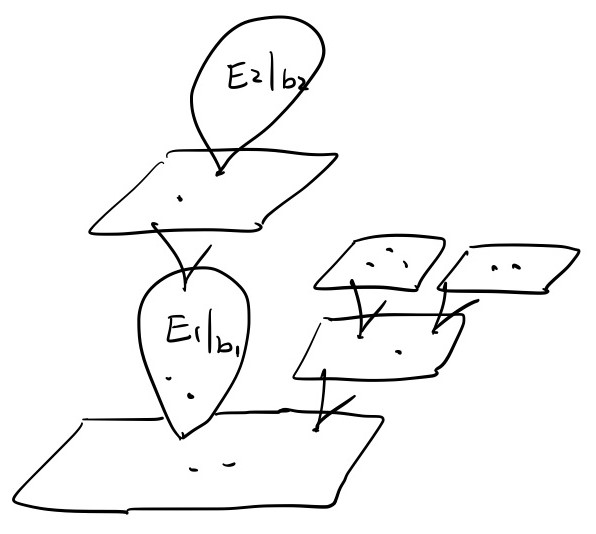
\includegraphics[scale=0.15]{x_fig}

by using the ``standard representations'' specified in Definition \ref{screennormalize_dfn}, 
we can view $x$ as literally a ``nodal'' space -- a space $X=\bigvee_{v\in V(T)}X_v$ obtained by wedging finitely many manifolds together (for the example here, a copy of $E_1|_{b_1}$, $E_2|_{b_2}$ and some copies of $S^d=\R^d\sqcup\{\infty\}$ are wedged together), together with $A$-many marked points scattered in it. 
Each component $X_v$, minus the lower node (``$\infty$''), now has a metric on it -- on the $S^d$-component it is the standard metric on $R^d$ and on the $E_1,E_2,E_{\mr{I}}$ components they are the metrics specified in Sections \ref{basic_sec},\ref{bracketbundle_sec}. 
Given a component $X_v$ of this nodal space and a point $p\in X_v$, if $p$ is not the lower node of $X_v$, we can talk about the ``ball of radius $r$ in $X_v$ centered at $p$'' to be given by the metric and the induced exponential map on $X_v$. 
If $p$ is the lower node, since each $X_v$ also has a specified ``identification with $\R^d$ near infinity'' near its lower node, we define the ``ball of radius $1/R$ centered at $p$'' to be $\{\infty\}\sqcup\R^d\backslash\D^d(R)$ under this identification. 
%\begin{itemize}
%\item $X_v\backslash\D^d(R)$ if $X_v=S^d$; 
%\item $X_v\backslash E_i(R)|_{b_i}$ if $X_v=E_i|_{b_i}$ for $i=1,2$, and $ls(>v)=\emptyset$; 
%\item $X_v\backslash \hat{E}_i(R)|_{b_i}$
%\end{itemize}

To construct $\psi_T(x,(\epsilon_e)_{e\in E(T)})$, 
for each node corresponding to $e\in E(T)$, we remove the ball of radius $r$ centered at the node from $X_{v_-(e)}$ and the ball of radius $1/R$ centered at the node from $X_{v_+e}$, where $r,R\ge0$ are chosen arbitrarily satisfying $r/R=\epsilon_e$, $r<r^{\min}(x;e)$, $R>R^{\max}(x;v_+(e))$; 
we then glue the two boundaries together, forming a new (maybe nodal) space with $A$-many marked points on it. This space, together with the marked points, represent an element in $\wt{C}_A$, which we define $\psi_T(x,(\epsilon_e)_{e\in E(T)})$ to be. 

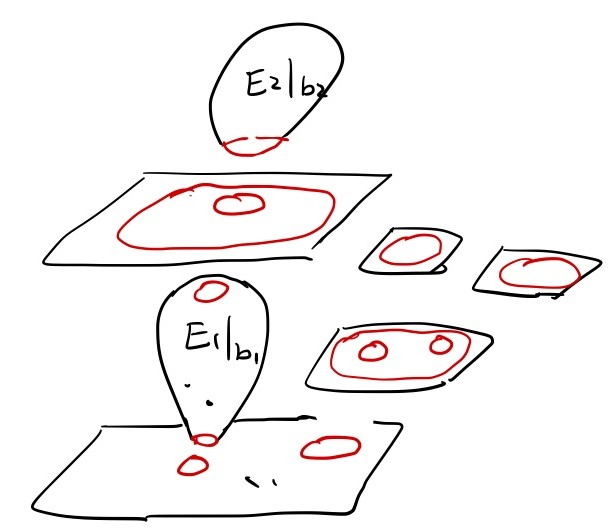
\includegraphics[scale=0.15]{xcut_fig}
\hspace{3cm}
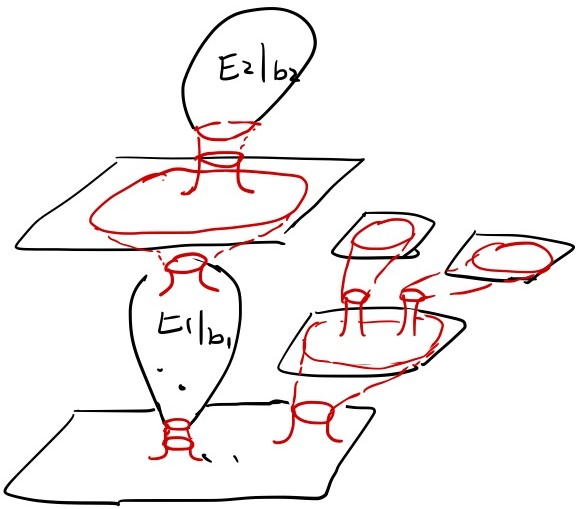
\includegraphics[scale=0.15]{xglue_fig}
 
This gives the definition of $\psi_T$. Since writing it down in fully formal terms is tedious and seems unnecessary, we will not do so here. 
The interested readers can write down the map in the term of formal formulas and the following corollary would be clear:  

\begin{crl}
The conditions \ref{psi2_item}, \ref{psi3_item} above follows immediately from the definition. 
\end{crl}

\begin{lmm}
$\psi_T$ is injective. 
\end{lmm}
\begin{proof}
\cmt{This follows immediately from the ``Riemannian center of mass'' notion in \cite{GroveKarcher}.}
\end{proof}

\begin{lmm}
Suppose $T_1,T_2\in\cT(A)$, and one of them can be obtained from the other by contracting some edges.  
\begin{itemize}
\item $\psi_{T_2}^{-1}(\tn{image}(\psi_{T_1})\cap\tn{image}(\psi_{T_2}))\subset\dom(T_2)$ is of the form 
$$\big\{\big(x,(\epsilon_e)_{e\in E(T_2)}\big)\in \dom(T_2)\subset S_{T_2}\times(\R^{\ge0})^{E(T_2)}\big|\,\forall\,e, \epsilon_e<\epsilon'_e(x)\big\},$$
where $\epsilon'_e(x)\le \epsilon^{\max}_{T_2;e}(x)$ are smooth functions on $S_{T_2}$. 
\item 
\begin{align*}
\psi_{T_1}^{-1}\circ\psi_{T_2}\big|_{\psi_{T_2}^{-1}(\tn{image}(\psi_{T_1})\cap\tn{image}(\psi_{T_2}))}:
\big\{\big(x,(\epsilon_e)_{e\in E(T_2)}\big)\in S_{T_2}\times(\R^{\ge0})^{E(T_2)}\big|\,\forall\,e, \epsilon_e<\epsilon'_e(x)\big\}\\
\longrightarrow
\big\{\big(x,(\epsilon_e)_{e\in E(T_1)}\big)\in S_{T_1}\times(\R^{\ge0})^{E(T_1)}\big|\,\forall\,e, \epsilon_e<\epsilon^{\max}_{T_1;e}(x)\big\}
\end{align*}
is given by: 
$$
\big(x,(\epsilon_e)_{e\in E(T_2)}\big)\longrightarrow \big( \psi_{T_1}(x,(...=0)), (\tn{smooth functions in }x, \{\epsilon_e'\}_{e'})_e \big)
$$
\end{itemize}
\end{lmm}

\begin{proof}

\end{proof}

\begin{rmk}
If we have used a different $i,j$ in Definition \ref{screennormalize_dfn}, and denote by $\psi'_T$ instead of $\psi_T$ the map thus obtained, then $(\psi'_T)^{-1}\circ\psi_T$ can be easily seen to also be a smooth map defined on an open subset of $\dom(T)$. So, the choices of $i,j$ in defining the standard representative does not matter for our purpose here. 
\end{rmk}




\subsection{Smoothing out one node}

Suppose $T\in\cT(A)$ and $e\in E(T)$. 
We construct a map 
$$\psi_{T;e}: \dom(T;e)\longrightarrow S_T\sqcup S_{T/e}.$$
Define $\psi_{T;e}|_{S_T\times 0}$ to map by the identity to $S_T$. 
%Now we define $\psi_{T;e}:\dom(T;e)-S_T\times0\to S_{T/e}$. 

For $x=\big(x_v\in C_{cld(v)\sqcup lp(v)}(ls(v))\big)_{v\in V(T)}$ and $\epsilon>0$, define 
$$\psi_{T;e}(x,\epsilon)=\big(y_v\in C_{cld(v)\sqcup lp(v)}(ls(v))\big)_{v\in V(T/e)}$$ 
as follows: 
take $y_{\tn{contr}^V_{T;e}(v)}=x_v$; it remains to define $$y_{[e]}\in C_{lp(v_+(e))\sqcup lp(v_-(e))\sqcup cld(v_+(e))\sqcup (cld(v_-(e))\backslash v_+(e))}(ls(v_-(e))+ls(v_+(e))).$$

Before going into the detail of this, we explain how intuitively $y_{[e]}$ is defined. It is obtained from $x_{v_-(e)}$ and $x_{v_+(e)}$ as follows: 

Take, arbitrarily, $R>R^{\min}(x;v_+(e))$ and $r<r^{\max}(x;e)$ such that $r/R=\epsilon$. 

Draw $x_{v_-(e)}$ and $x_{v_+(e)}$ as below: 

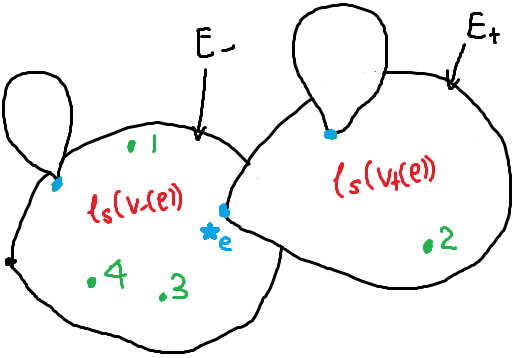
\includegraphics[scale=0.5]{yedfn1_fig}

where $x_{v_-(e)}$ (resp. $x_{v_+(e)}$) is the configuration of green and blue points on $ls(v_-(e))$ (resp. $ls(v_+(e))$). 
Here the space where the marked points lie on, denoted by $E_\pm$, is the fiber of the bundle $ls(v_\pm(e))$ on which $x_{v_\pm(e)}$ lies, if $ls(v_\pm(e))\neq\R^d$; if $ls(v_{\pm}(e))=\R^d$, then $E_\pm=\R^d$, and the positions of points on it are given by $x'_{v_\pm(e)}$. 

Next, we cut off a disk of radius $r$ in $E_-$, centered at $\star_e$. Here, if $E_-\neq\R^d$, ``radius $r$'' is made sense of by the exponential map. 

We also cut off a neighborhood of $\star_e$ in $E_+$. This neighborhood is the one identified with $\R^d\backslash\D^d(R)$ via a ``trivialization at $\infty$'' of $ls(v_+(e))$. This ``trivialization at $\infty$'' depends on $ls(v_+(e))$ and $ls(>v_\pm(e))$: if $ls(v_+(e))=\R^d$, then it is the standard trivialization on $\R^d$; if $ls(v_+(e))=\pi_i$ and $ls(>v_+(e))=\emptyset$, then it is $\tau'_i$; if $ls(v_+(e))\neq\R^d$ and $ls(>v_-(e))=\{\pi_1,\pi_2\}$, then it is induced from the trivializations $\hat\tau'_i$ or $\tau_\rI$ defined in Section \ref{tauEI_subsec}. 

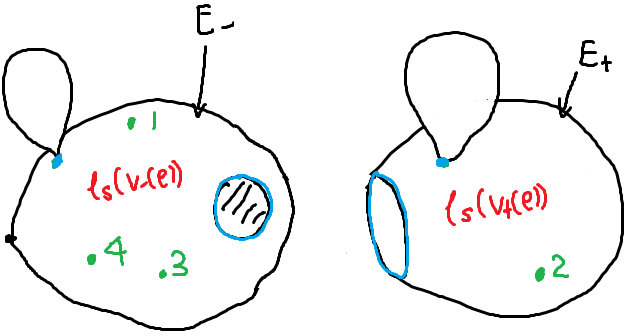
\includegraphics[scale=0.5]{yedfn2_fig}

Last, we glue this two pieces together to form $y_{[e]}$. Notice that the result doesn't depend on the choices of $r,R$, as long as they satisfy the required conditions:
$R>R^{\min}(x;v_+(e))$, $r<r^{\max}(x;e)$, and $r/R=\epsilon$. 

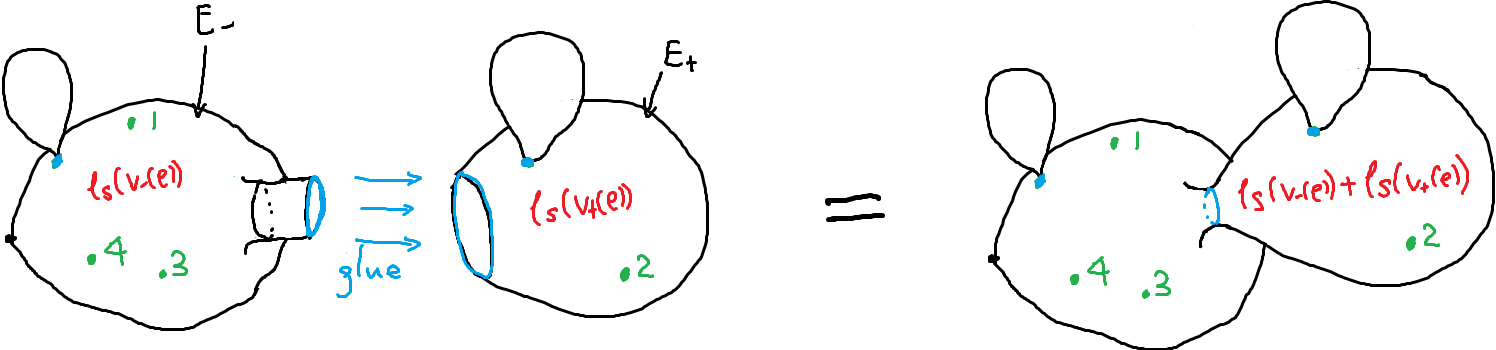
\includegraphics[scale=0.5]{yedfn3_fig}


The above is the intuition of constructing $y_{[e]}$. Now, the detailed description of defining $y_{[e]}$: 

\begin{itemize}
\item If $ls(v_+(e))=\R^d, ls(v_-(e))\neq\R^d$:
let $E_e$ be the fiber of $ls(v_-(e))$ on which $x_{v_-(e)}$ lies;
let $\star_e\in E_e$ be the location of the marked point $v_+(e)$ in the configuration $x_{v_-(e)}$; 
%let $b_e=ls(v_-(e))(x_{v_-(e)})$ be the point in the base of $ls(v_-(e))$ over which $\star_e$ lies; 
then, 
$y_{[e]}$ is obtained from $x_{v_-(e)}$ by first removing the marked point $v_+(e)\in cld(v_-(e))$ and then adding the marked points in $cld(v_+(e))\sqcup lp(v_+(e))$ to $E_e$, as the image of $x'_{v_+(e)}$ under the map
$$(\R^d)^{cld(v_+(e))\sqcup lp(v_+(e))}\xrightarrow{(\exp_{\star_e},\ldots,\exp_{\star_e})\circ\tn{ scaling by }\epsilon}(E_e)^{cld(v_+(e))\sqcup lp(v_+(e))}.$$
\item If $ls(v_+(e))=\R^d, ls(v_-(e))=\R^d$: let $\star_e\in \R^d$ be the location of the marked point $v_+(e)$ in the configuration $x'_{v_-(e)}$; then, 
a representative of $y_{[e]}$ is obtained from $x'_{v_-(e)}$ by first removing the marked point $v_+(e)\in cld(v_-(e))$ and then adding the marked points in $cld(v_+(e))\sqcup lp(v_+(e))$ to $\R^d$, as the image of $x'_{v_+(e)}$ under the map
\begin{align*}
(\R^d)^{cld(v_+(e))\sqcup lp(v_+(e))}&\longrightarrow(\R^d)^{cld(v_+(e))\sqcup lp(v_+(e))}\\
(w_v\in\R^d)_{v\in cld(v_+(e))\sqcup lp(v_+(e))}&\longrightarrow\big(\epsilon\cdot w_v+\star_e\big)_{v\in cld(v_+(e))\sqcup lp(v_+(e))}.
\end{align*}
\item If $ls(v_+(e))=\pi_1$, $\pi_2$ or $\pi_\rI$, $ls(v_-(e))=\R^d$:  
let $\star_e\in\R^d$ be be the location of the marked point $v_+(e)$ in the configuration $x'_{v_-(e)}$; 
let $E_e$ be the fiber of $ls(v_+(e))$ in which the configuration $x_{v_+(e)}$ lies; then, 
$y_{[e]}$ is obtained from $x_{v_+(e)}$ by adding the marked points in $cld(v_-(e))\sqcup lp(v_-(e))$ to $E_e$, as the image of $x'_{v_-(e)}$ under the map
\begin{align*}
(\R^d\backslash\D^d_{\star_e}(r^{\max}(x;e)))^{cld(v_-(e))\sqcup lp(v_-(e))}&\longrightarrow(E_e)^{cld(v_-(e))\sqcup lp(v_-(e))},\\
(w_v\in\R^d)_{v\in cld(v_-(e))\sqcup lp(v_-(e))}&\to (\tau|_{E_e})^{-1}\big(1/\epsilon\cdot(w_v+\star_e)\big)_{v\in cld(v_-(e))\sqcup lp(v_-(e))}
\end{align*}
where 
$$\tau=\begin{cases}
\tau'_i, \tn{ if }ls(v_+(e))=\pi_i, i=1 \tn{ or } 2, \tn{ and } ls(>v_+(e))=\emptyset \\
\hat\tau'_i, \tn{ if }ls(v_+(e))=\pi_i, i=1 \tn{ or } 2, \tn{ and } ls(>v_+(e))=\{\pi_{3-i}\} \\
\tau_\rI, \tn{ if }ls(v_+(e))=\pi_\rI. 
\end{cases}$$
\item  If $ls(v_-(e))=\pi_{i}$ and $ls(v_+(e))=\pi_{3-i}$ for  $i=1$ or $2$:  
let $E^-_e$ (resp. $E^+_e$) be the fiber of $\pi_{i}$ (resp. $\pi_{3-i}$) in which the configuration $x_{v_-(e)}$ (resp. $x_{v_+(e)}$) lies; 
let $\star_e\in E_e^-$ be the location of the marked point $v_+(e)$ in the configuration $x_{v_-(e)}$. 
Then, 
\begin{itemize}
\item if $\star_e\in E_{i}(3)$, 
then $y_{[e]}$, as a configuration of points on $\pi_\rI$, lies on the fiber over
$(\star_e,\pi_{3-i}(x_{v_+(e)}),\epsilon)\in E_i(3)\times B_{3-i}\times(0,\rho)$; 
\item if $\star_e\in E_{i}-\sigma_{i}(B_i)-E_{i}(2)$,  
write 
$$\tau'_i(\star_e)=\big(\pi_i(x_{v_-(e)}),l,\theta\big)\in B_i\times \R^d\backslash\D^d(3),$$
where $(l\in[3,\infty), \theta\in S^{d-1})$ is the polar coordinate of the $\R^d\backslash\D^d(3)$-factor,
then $y_{[e]}$, as a configuration of points on $\pi_\rI$, lies on the fiber over
\begin{align*}
\big((-1)^{i-1}\theta,\pi_i(x_{v_-(e)}),\pi_{3-i}(x_{v_+(e)}),\gamma^{-1}(x,y)\big)&\in S^{d-1}\times B_i\times B_{3-i}\times(0,\rho)\times[-\frac{1}{2},\frac{1}{2}]\\
&%\stackrel{\tn{switching factors}}
{\approx} S^{d-1}\times[-\frac{1}{2},\frac{1}{2}]\times B_1\times B_{2}\times(0,\rho)
\end{align*}
where $x=1/l, y=\epsilon$, and
$\gamma:(0,\rho)\times[-1/2,1/2]\to\R^2$ is the map in Section \ref{second_subsubsec}, defined right under the second picture in that section. 
\end{itemize}
Recall in Section \ref{EI_subsec} we constructed $E_\rI$ by doing surgery on $E_1$ and $E_2$, so parts of $E_\rI$ are naturally identified with parts of $E_1$ and $E_2$.
We define $y_{[e]}$ by putting together the marked points in $x_{v_-(e)}$ and $x_{v_+(e)}$, which are viewed as points in $E_\rI$ under this identification. 
\end{itemize}

This completes the definition of $\psi_{T;e}$. 
It is easy to be convinced that  $$\psi_{T;e}|_{\tn{dom}(T;e)-S_T\times0}:\tn{dom}(T;e)-S_T\times0\to S_{T/e}$$
is smooth. 
\cmt{Maybe re-write the above in a better way to make this obvious.}

To show $\psi_{T;e}$ has a smooth inverse on a sufficiently small neighborhood of $S_T$: in the case $ls(>v_-(e))$ is non-empty or $ls(v_-(e))=\R^d$, this is clear (the case $ls(v_+(e))=\pi_i$, $ls(v_-(e))=\pi_{3-i}$ follows by how the bracket bundle is constructed); in the case $ls(>v_-(e))$ is empty and $ls(v_-(e))\neq\R^d$, all the difficulty here is, given a collection of points $x_1,\ldots,x_n$ in a small region on a manifold $M$, whether there is a unique point $p\in M$ nearby such that $x_1,\ldots,x_n$ can be obtained from a configuration of points in $T_pM$ by exponential map at $p$. This is precisely the definition of the Riemannian center of mass in \cite{GroveKarcher}. The uniqueness of $p$ is given by \cite[Proposition 3.1]{GroveKarcher}. 


\subsection{Smoothing out multiple nodes}

Given $T\in\cT(A)$, and an (arbitrary) order on $E(T)$, 
%we write $E(T)=\{e_1,\ldots,e_m\}$. 
we define $\psi_T:\tn{dom}(T)\to\wt{C}_A$  by smoothing out the nodes one by one. 
\cmt{From here to just above Lemma \ref{psicommute_lmm} can be skipped on first reading.}
More precisely, given $$\big((x_v)_{v\in V(T)},(\epsilon_{e})_{e\in E(T)}\big)\in\tn{dom}(T)=S_T\times(\R^{\ge0})^{E(T)},$$ 
$\psi_T\big((x_v),(\epsilon_{e})\big)$ is determined by the following inductive process: 
first, write 
$$E'(T)=\{e\in E(T)\big|\,\epsilon_e\neq0\}\subset E(T),$$
then: 
\begin{itemize}
\item Start with $T_0=T$, $E'(T)$, the induced order on $E'(T)$, and $X_0=\big((x_v)_{v\in T},(\epsilon_{e})_{e\in E'(T)}\big)$. 
\item Given $T_i\in\cT(A)$, a subset $E'(T_i)\subset E(T_i)$, an order on $E'(T_i)$,and $$X_i=\big((x_{i,v})_{v\in V(T_i)}\in S_{T_i},(\epsilon_{e}\in\R^{>0})_{e\in E'(T_i)}\big),$$ we construct $T_{i+1}$, $E'(T_{i+1})$, an order on $E'(T_{i+1})$, and $X_{i+1}$: 
\begin{itemize}
\item Let $e'\in E'(T_i)$ be the first element of $E'(T_i)$, then
$$T_{i+1}=T_i/e',\qquad E'(T_{i+1})=\tn{contr}^E_{T_i;e'}\big(E'(T_i)\backslash\{e'\}\big)$$
and the order on $E'(T_{i+1})$ is induced from the order on $E'(T_i)$ and $\tn{contr}^E_{T_i;e'}$.  
\item For all $v\in V(T_i)$, $x_{i+1,\tn{contr}^V_{T_i;e'}}=x_{i,v}$. 
\item $x_{i+1,[e']}=\psi_{T_i;e'}\big((x_{i,v})_{v\in V(T_i)},\epsilon_{e'}\big)$.
\item For all $e\neq e'\in E'(T_i)$, if $\{v_-(e),v_+(e)\}\cap \{v_-(e'),v_+(e')\}=\emptyset$, then $\epsilon_{\tn{contr}^E_{T_i;e'}(e)}=\epsilon_e$. 
\item It remains to determine $\epsilon_{\tn{contr}^E_{T_i;e'}(e)}$ for other $e\neq e'\in E'(T_i)$: 
\begin{itemize}
\item If $ls(v_-(e'))=\R^d$, $ls(v_+(e'))\neq\R^d$, then, for $e\neq e'\in E(T_i)$: 
$$\begin{cases}
v_-(e)=v_+(e')\implies \epsilon_{\tn{contr}^E_{T_i;e'}(e)}=\epsilon_e,\\
v_-(e)=v_-(e')\implies \epsilon_{\tn{contr}^E_{T_i;e'}(e)}=\epsilon_e/\epsilon_{e'},\\ 
v_+(e)=v_-(e')\implies \epsilon_{\tn{contr}^E_{T_i;e'}(e)}=\epsilon_e\cdot\epsilon_{e'}.
\end{cases}$$
\item If $ls(v_+(e'))=\R^d$, and either $ls(v_-(e'))\neq\R^d$ or 
$$ls(v_-(e'))=\R^d, v_+(e)\tn{ is not the out-most marked point in }x_{i,v_-(e)},$$  
then, for $e\neq e'\in E(T_i)$: 
$$\begin{cases}
v_-(e)=v_+(e')\implies \epsilon_{\tn{contr}^E_{T_i;e'}(e)}=\epsilon_e\cdot\epsilon_{e'},\\
v_-(e)=v_-(e')\implies \epsilon_{\tn{contr}^E_{T_i;e'}(e)}=\epsilon_e,\\ 
v_+(e)=v_-(e')\implies \epsilon_{\tn{contr}^E_{T_i;e'}(e)}=\epsilon_e.
\end{cases}$$
\item If $ls(v_-(e'))=ls(v_+(e'))=\R^d$ and $v_+(e)$ is the out-most marked point in $x_{i,v_-(e)}$, then...
\cmt{not yet written; would be very annoying to write; you can probably see what I want to say; should find another way to write these, or change the second bullet in Definition  \ref{screennormalize_dfn}}
\item If $ls(v_-(e'))=\pi_i$, $ls(v_+(e'))=\pi_{3-i}$: let $\star_e\in E_i$ be the position of the marked point $v_+(e')$ in the configuration $x_{i,v_-(e)}$.  
\begin{itemize}
\item If $\star_e\in E_i(2)$, then, for all $e\neq e'\in E(T_i)$, $\epsilon_{\tn{contr}^E_{T_i;e'}(e)}=\epsilon_e$.
%\item if $\star_e\in E_i(3)-E_i(2)$, then...\cmt{not written yet} 
\item If $\star_e\in E_i-\sigma_i(E_i)-E_i(2)$: let $g_i:E_i-\sigma_i(B_i)\to \R^{\ge1}$ be the function defined in Section \ref{trivEI1_subsubsec}. 
Then, 
$$\begin{cases}
v_-(e)=v_+(e')\implies \epsilon_{\tn{contr}^E_{T_i;e'}(e)}=\epsilon_e,\\
v_-(e)=v_-(e')\implies \epsilon_{\tn{contr}^E_{T_i;e'}(e)}=\epsilon_e\cdot g_i(\star_e)/3,\\ 
v_+(e)=v_-(e')\implies \epsilon_{\tn{contr}^E_{T_i;e'}(e)}=\epsilon_e\cdot3/g_i(\star_e).
\end{cases}$$
\end{itemize}
\end{itemize}
\end{itemize}
\item Define $\psi_T\big((x_v),(\epsilon_e)\big)=X_{|E'(T)|}$. 
\end{itemize}
This completes the definition of $\psi_T$. 

\begin{lmm}\label{psicommute_lmm}
$\psi_T$ doesn't depend on the choice of order on $E(T)$. 
\end{lmm}
\begin{proof}
\cmt{If I have not made a mistake (which I probably have...), this should be true and easy to verify. The definitions in Section \ref{normalization_subsec} are designed for this lemma to hold.}
\end{proof}

\begin{crl}
For $T\neq T'\in \cT(A)$, the transition map $\psi_{T'}^{-1}\circ\psi_{T}|_{\psi_T^{-1}(\tn{image}(\psi_T)\cap\tn{image}(\psi_{T'}))}$ is smooth. 
Therefore, $\wt{C}_A$ is a well-defined smooth manifold with boundary and corners. For $T\in\cT(A)$, $S_T\subset \wt{C}_A$ is a codimension-$|E(T)|$ stratum. 
\end{crl}

If $A'\subset A$ is a finite subset, then we have an obviously-defined forgetful map $f_{A,A'}:\wt{C}_A\to\wt{C}_{A'}$. 

\begin{lmm}
$f_{A,A'}:\wt{C}_A\to\wt{C}_{A'}$ is smooth. \cmt{proof not yet written. Note that the forgetful maps are not smooth in the sense of Joyce's paper ``Manifold with corners''; smoothness here means ``weakly smooth'' there.}
\end{lmm}


\begin{thebibliography}{9}
\bibitem{GroveKarcher} K. Grove and H. Karcher, {\it How to Conjugate $C^1$-Close Group Actions}, Math. Z., 1973
\end{thebibliography}


\end{document}